\documentclass[11pt,a4paper]{article}
\usepackage{hyperref}
\usepackage{color}
\usepackage{amsmath, amsthm, amssymb, amsfonts, verbatim}
\usepackage{graphicx}
\usepackage[table,x11names]{xcolor}
\usepackage{geometry}
\usepackage{subcaption}

\title{Assessing glymphatic transport velocities by adjoint methods}

\renewcommand{\comment}[1]{\textcolor{red}{#1}}

\newcommand{\kam}[1]{\textcolor{blue}{#1}}

\author{Lars Magnus Valnes, Sebastian K. Mitusch, Geir A. Ringstad, \\ 
Per Kristian Eide, Simon W. Funke, Kent-Andre Mardal }


\begin{document}
\maketitle

\begin{abstract}
bla bla 
\end{abstract}
\section{Introduction}

A novel pathway of the brain's metabolism system called the paravascular pathway, because it runs in parallel with 
vasculature system in a surrounding compartment,  
was discoved in 2011~\cite{iliff2012paravascular}. 
%Later it was found that this system is particularly active during sleep~\cite{xie2013sleep}.  
It has been proposed that this pathway plays an important role in the clearance of waste
from the brain and hereby a malfunction of this system is linked to  the development of dementia such as Alzheimer's and Parkinson's diseases. That is, 
the lymphatic system plays a crucial role in waste clearance in the rest of our body, but there are no lymph vessels inside
the brain. As such, the metabolic process of the brain is not well understood and this is surprising since the brain is a very 
energy demanding organ (about 10 times as demanding as the average organ). The circulatory system of the paravascular pathway 
has therefore been named the glymphatic system~\cite{jessen2015glymphatic} as it has a similar role as the well-known lymphatic system and because the glia cells 
are crucial in this system.  
The glymphatic system remains controversial and modeling attempts
has so far mostly failed to explain the biomechanics of the system~\cite{asgari2016glymphatic, holter2017interstitial, smith2017glymphatic}\kam{Lars: vi trenger flere her}. A proper biomechanical 
understanding of the pathway has significant potential because
dementia such as Alzheimer´s and Parkinson´s diseases are
associated with accumulation of metabolic waste such as
amyloid-beta and CSF-tau.  

In \cite{ringstad2018brain} brain-wide distribution of MRI-contrast was demonstrated during 24 hours after lumbar contrast injection. Brain-wide distribution by diffusion alone was deemed unlikely by the authors (some of which are part 
of this study as well). The argument was based on analytical considerations where it was calculated that 50\% contrast enrichment would occur after 
55 hours using the error function which is valid for planar diffusion. However, 
the surface of the brain is folded and is around five times larger than 
a corresponding surface of a ball with the same volume. Hence, 
a more rigorous modeling attempt is warrented. A complicating factor
is however that the contrast in the surrounding CSF is heterogenous
and changes significantly during the 24 hours of the investigations. 
Furthermore, images were obtained only at a few time-points during the investigations in \cite{ringstad2018brain}.  

The pioneering works of Sykov{\'a} and Nicholson~\cite{sykova2008diffusion} demonstrated
that diffusion was a governing transport mechanism in the brain and estimated to be on the order
of XXX. This is confirmed with DTI where values of young and healthy are typically around XXX
while values in dementia typically are XXX \kam{Geir vet du dette?}. Of course diffusion coefficient 
measured by DTI at a time-scale of XXX \kam{tall her} may not be representative for the process on a
longer time-scale, at least if the paravascular pathway plays an important role. The fact that the vasculature  occupy around 3\% of the brain volume 
and the paravascular network is substatantially smaller potentially render it invisible at the short time-scales of a DTI investigation 
while it may still be effective on longer time scales.   


Our purpose in this paper is to attempt a more rigorous methodology 
for assessing the apparent diffusion process where
the complex geometry of the brain is taken into account. The approach 
we will take is to solve a PDE constrained optimization problem 
via adjoint methods. As such we need to assess the sensitivity of
the approach with respect important parameters such as to regularization parameters, noise levels, 
time resolution to determine whether this approach is a viable method
to obtain parameters involved time-scales beyond those of the MRI aquisition.     



\subsection*{MRI Data}
\begin{figure}
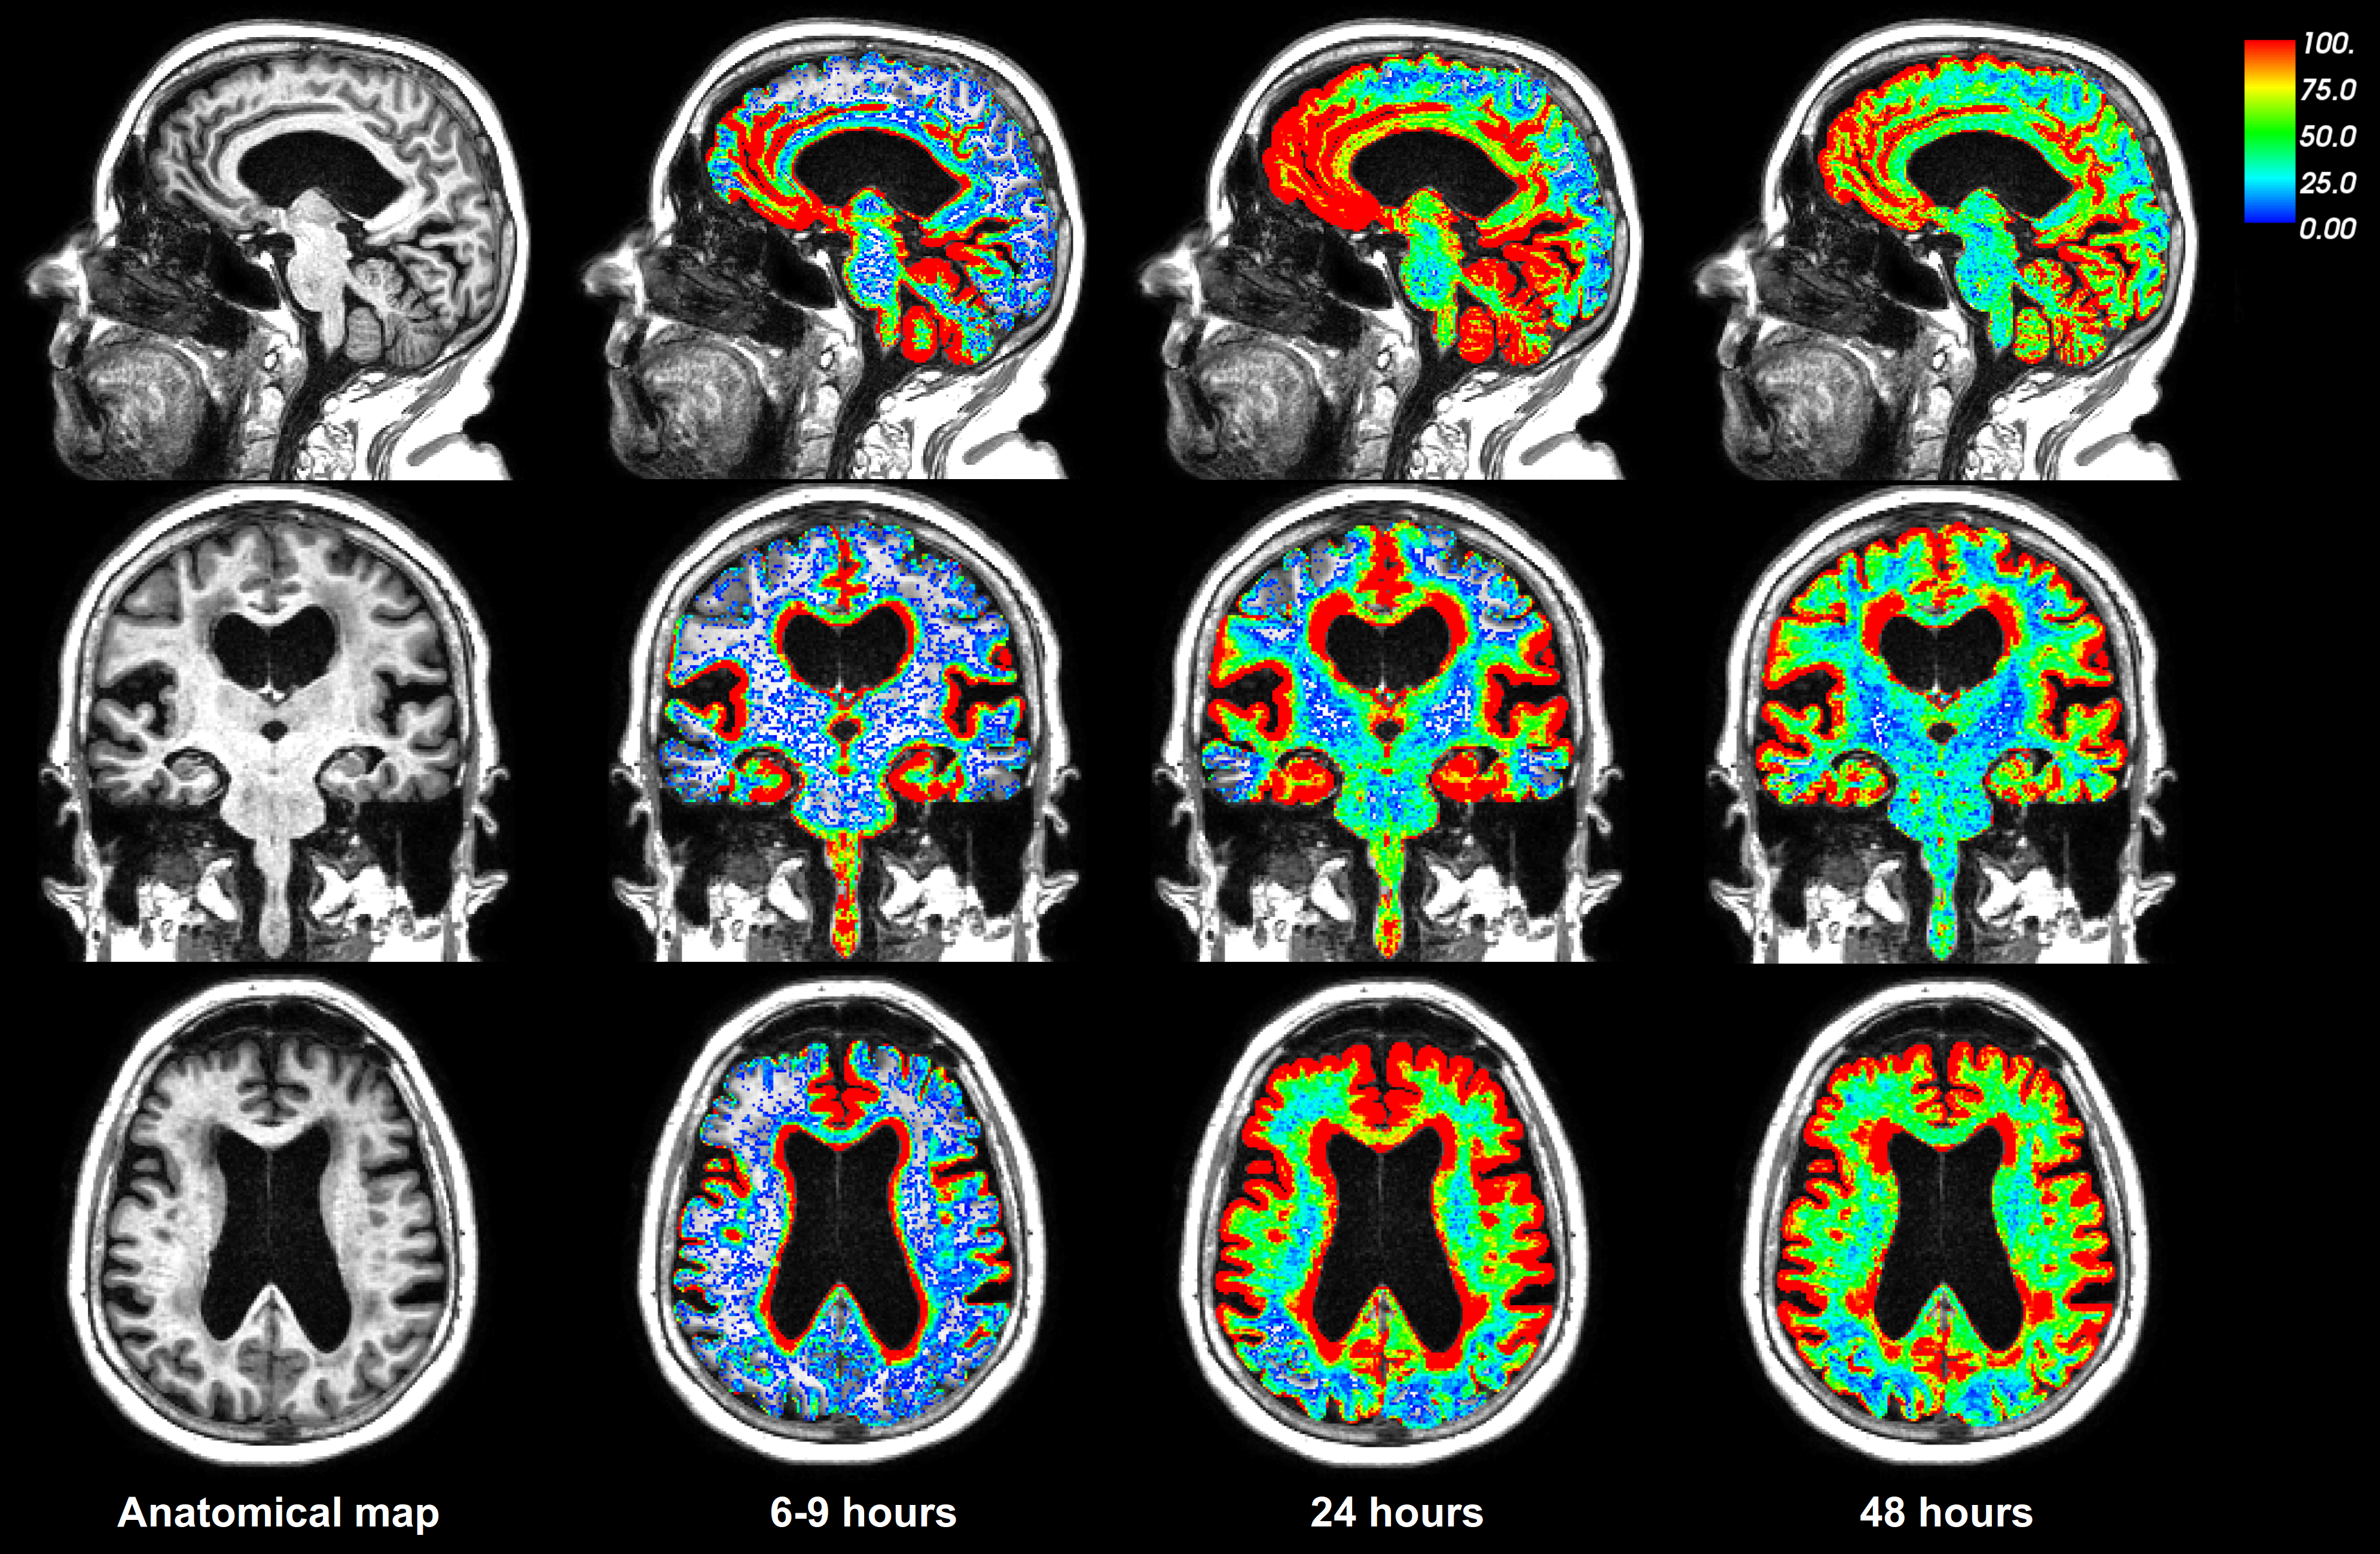
\includegraphics[width=0.95\textwidth]{PatID-68-new-100.png} 
\caption{Shows the percentage intensity increase from baseline at different observation times. The colorbar was restricted to the range $(0,100)$ }
\label{fig1} 
\end{figure}

\begin{figure}
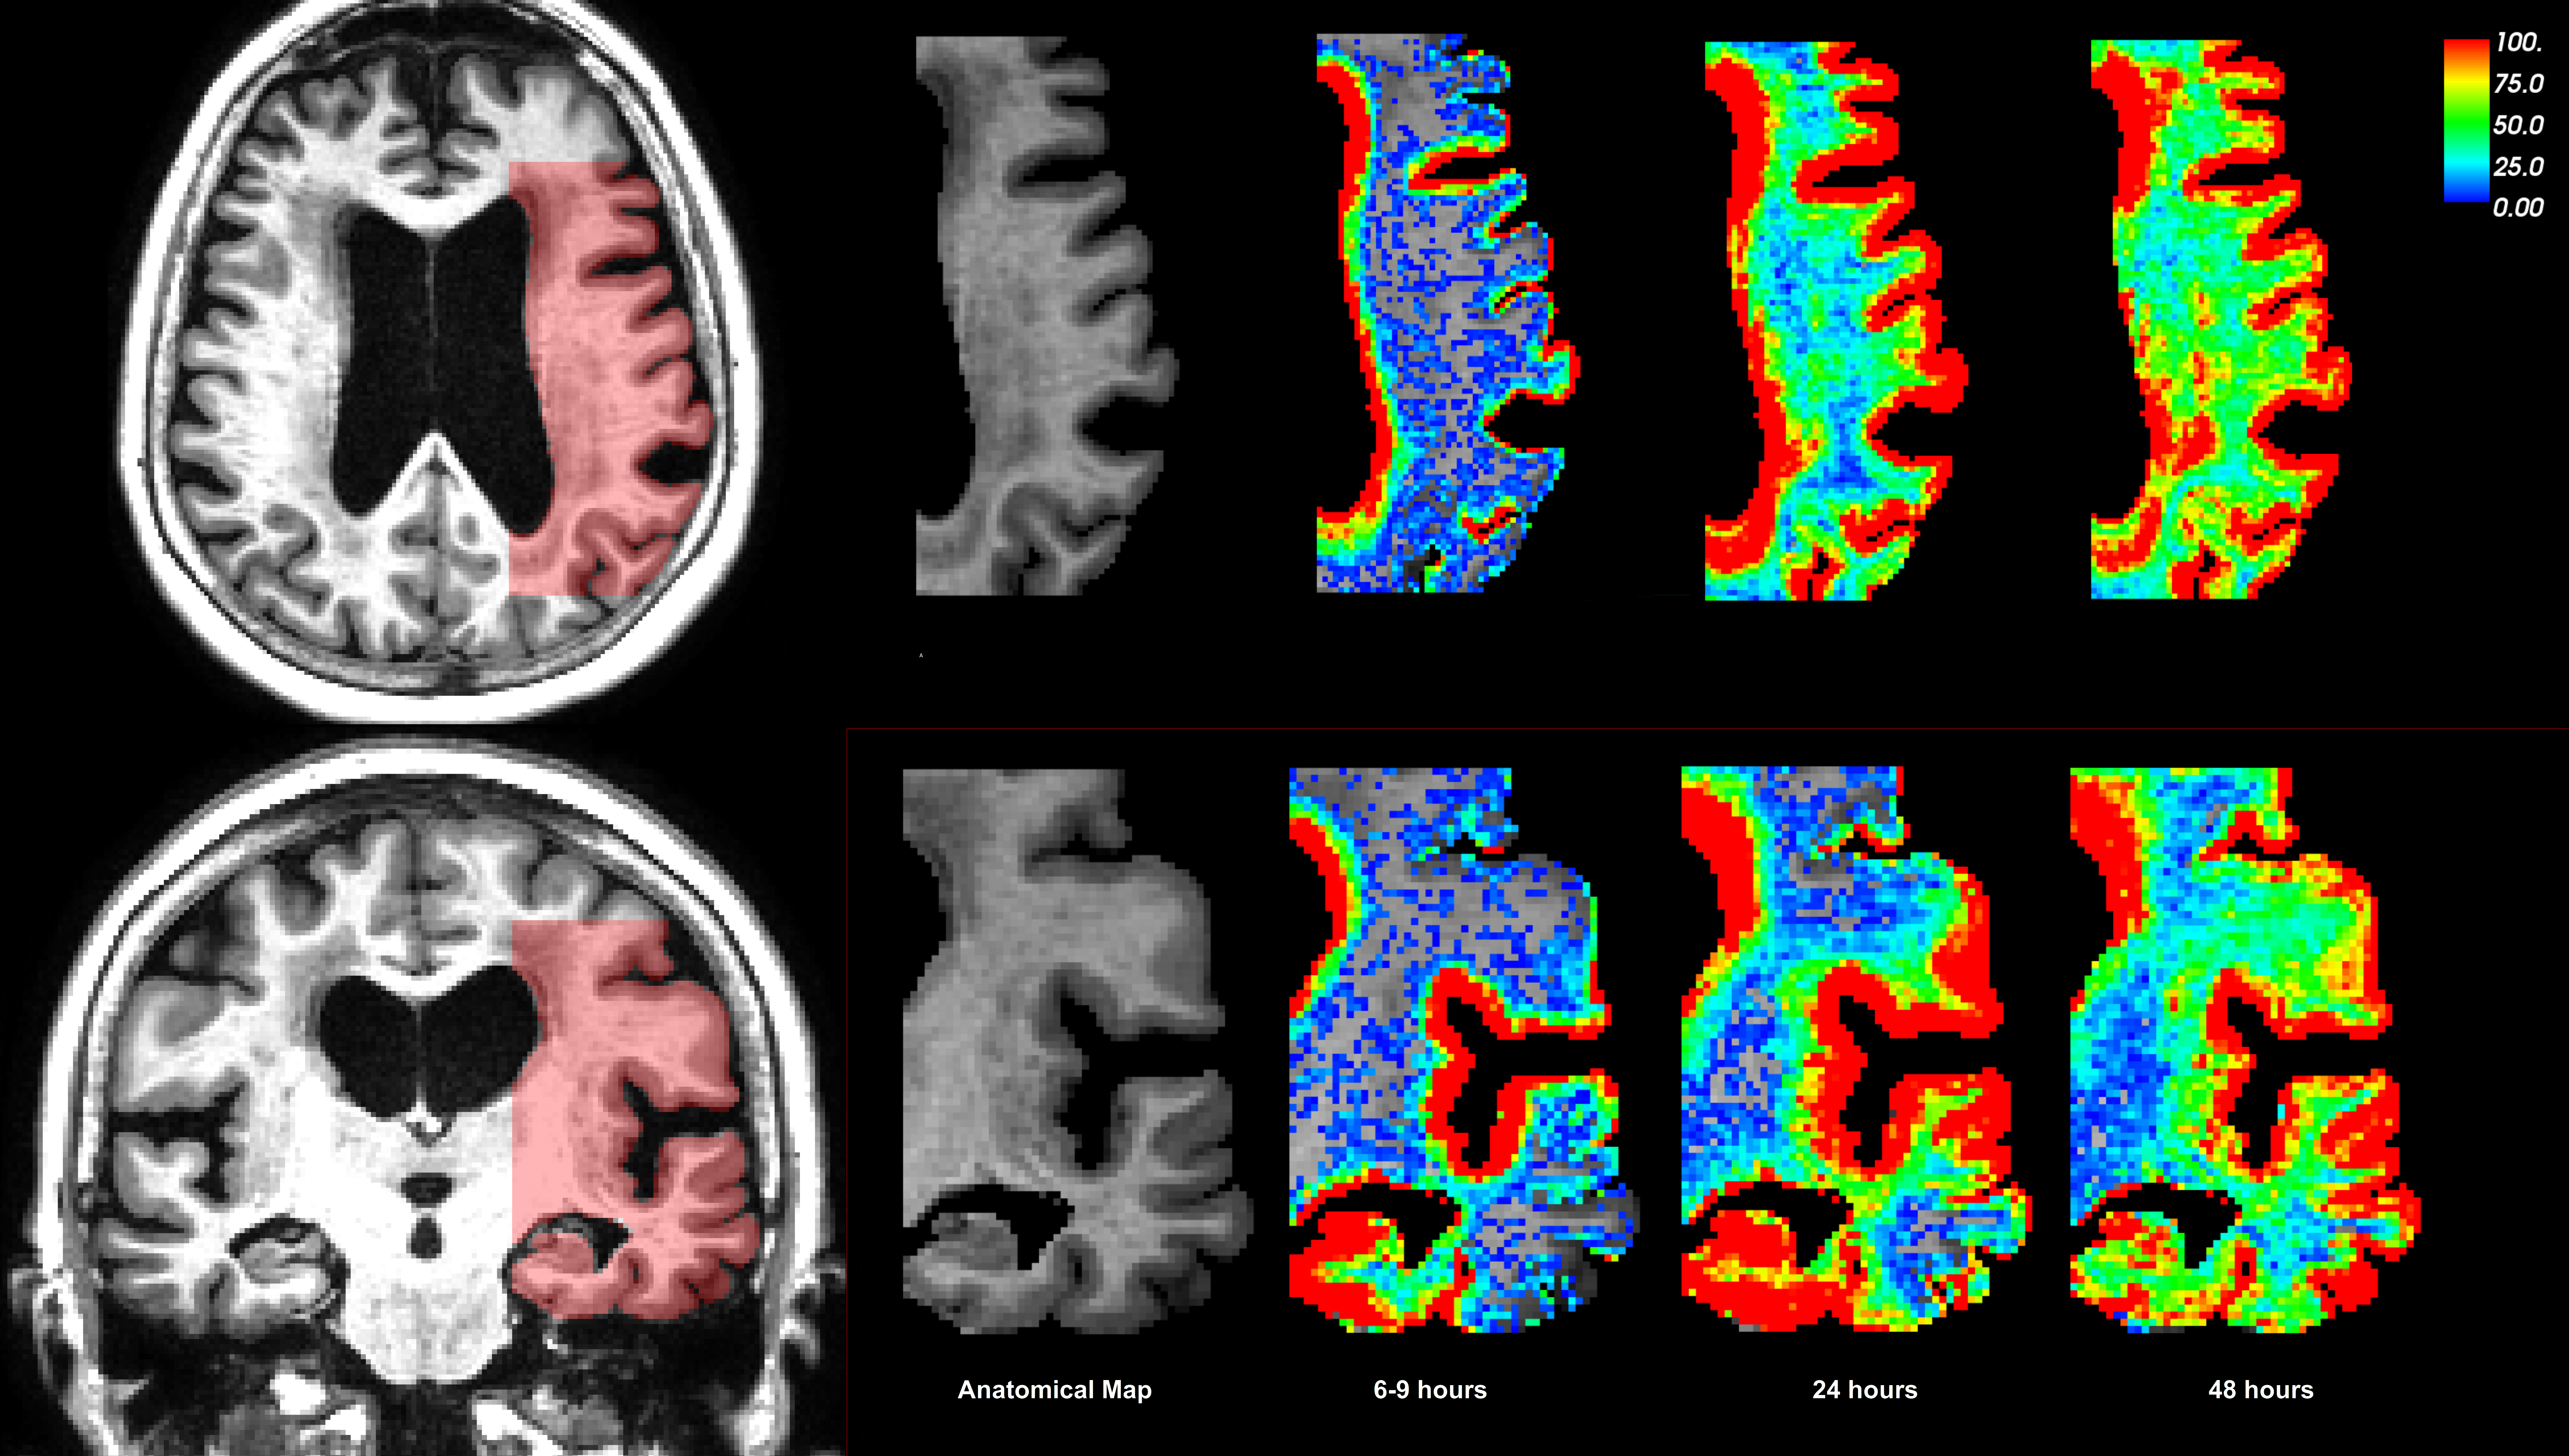
\includegraphics[width=0.95\textwidth]{Zoom-PatID-68.png} 
\caption{Shows the percentage intensity increase from baseline at different observation times in the slice (marked red in the left panel) used in the subsequent analysis.The colorbar was restricted to the range $(0,100)$}
\label{fig2} 
\end{figure}
Figure~\ref{fig1} shows the distribution of tracers during 24 hours, see also~\cite{ringstad2018brain} for further information on the imaging procedure.   
Our data (not all shown) consist of a total of 10 MRI observations, including a baseline MRI taken before tracer was injected. The observation points are distributed with 5 observations within 1-2 hours after injection, 1 observation in the timeframes 2-4 hours, 6-9 hours, 24 hours and 48 hours. 
Figure~\ref{fig2} shows the slice selected for our computations. 
The software Freesurfer was used to segment and align each of the observations, which made it possible to estimate voxelwise intensity increase. 



\subsection*{Mathematical Model}
In order to estimate the apparent diffusion coefficient involved in the contrast transportation shown 
in Figure~\ref{fig1} we assume that the process can be modeled by a diffusion equation and  
solve a PDE constrained optimization problem where
the contrast distribution, boundary conditions, and apparent
diffusion coefficient are solved for by optimizing with
respect to the observed contrast distribution. As such, enhanced transportation because of effects such as
dissipation would result in an apparent diffusion coefficient larger than that predicted by DTI.  
The objective function was defined as 
\begin{equation}
\min_{u,g} F = \quad \sum\limits_i\sp{n} \int\limits_{\Omega} |u(t_i) - u_{obs}(t_i)| \mathrm{d}\Omega + \frac{\alpha}{2} \int\limits_{0}\sp{T} || g ||_{L\sp{2}(\partial\Omega)} \mathrm{d}t + \frac{\beta}{2} \int\limits_{0}\sp{T} || \dot{g} ||_{L\sp{2}(\partial\Omega)}\mathrm{d}t 
\label{EQ::objf}
\end{equation}
subject to   
\begin{equation}
\begin{aligned}
\frac{\partial u}{\partial t} = \nabla \cdot  D_i \nabla u \qquad \text{in} \qquad \Omega \times \left\lbrace 0 , T \right)  \\
u=g(t) \qquad \text{on} \qquad \partial\Omega  \times \left\lbrace 0 , T \right) 
\end{aligned}
\label{Eq::PDE}
\end{equation}
Here, $u$ is the contrast distribution, $D_i$ is the apparent diffusion 
coefficient, and $g$ is the boundary condition. Furthermore,  
the domain $\Omega$ contains three sub domains, each with a different diffusion coefficient. We denote the Cerebral Spinal fluid (CSF) domain as $\Omega_1$, the grey matter as $\Omega_2$ and the white matter as $\Omega_3$. The apparent
diffusion constant is assumed constant within the CSF, grey and 
white matter but each region may have different constants.  
The $\alpha$ and $\beta$ parameters are regularization parameters 
and $u_{obs}$ are observations at certain time-points. 

\section*{Implementation}
The code used the FEniCS project to solve the PDE, using backwards Euler time discretization and first order continuous Galerkin finite elements. The linear problem was solved using GMRES, and the matrix was stored in the solver. 
The module dolfin adjoint ~\cite{farrell2013automated} \kam{correct ref?} was used to solve the PDE constrained optimization problem with the L-BFGS-B algorithm in the python module scipy. The convergence criteria for the minimization was set so that $max\lbrace | proj x_i | , \quad i = 1, .., N \rbrace \leq gtol=1.0e-1$ where $ proj x_i$ is the i-th component of the projected gradient. {\color{red} see scipy }.  

The implementation used the first observation as initial conditions of Eq.\ref{Eq::PDE}. Then for each timestep, the next observation was used as the initial value for boundary control $g$. The boundary control was imposed on the external boundary for the domain $D_{\Omega_1}$. 

The observations $u_{obs}$ have a fixed time-point $t_i$, these time-points may not overlap with the time discretization in the forward problem $t_j$. Therefore, after each time step $dt$ in Eq\ref{Eq::PDE}, it was checked if the time step contained the next observation. If it did, then a linear interpolation of the  current solution $u(t_j)$ and previous solution $u(t_{j-1})$ was used approximate the solution at time $t_i$. The linear interpolation was given as  
\begin{equation}
\label{observation:interpolation}
u(t_i) \approx \frac{\Delta t}{dt} u(t_{j-1}) + \frac{dt - \Delta t }{dt} u(t_{j}), \quad t_i \in \lbrace t_{j-1}, t_j \rbrace
\end{equation}
with $\Delta t = t_k-t_i $.  

The initial values of the diffusion coefficients in the optimization algorithm $(D_{CSF}, D_{GM}, D_{WM})=$  $(1, 1, 1)$. However, to increase the convergence rate, $D_{CSF}$ was scaled with $100$. 
The noise susceptibility was tested by adding an uniform distribution noise term to the observations. The noise term was constructed using numpy.random and adjusted so that noise range becomes $\lbrace -n_{amp} , n_{amp} \rbrace $, with $n_{amp}$ defined as noise amplitude. 

This work was performed on the Abel Cluster, owned by the University of Oslo and Uninett\textbackslash Sigma2, and operated by the Department for Research Computing at USIT,the University of Oslo IT-department. \url{http://www.hpc.uio.no/} 
\subsection*{Contrast concentration - Image Intensity Relation}
Below, we briefly describe the relationship between the imaging intensity 
seen in Figures \ref{fig1} and \ref{fig2} and the underlying contrast 
concentration. We remark that we use a notation common in medical literature and here two letter symbols are common. Hence, below we will use two letter symbols such as $TE$ and $TR$ to keep the notation consistent the presentation of (reference \cite{GOWLAND}, \cite{MPRAGE}).   
The tracer concentration $c$ causes the longitudinal(spin-lattice) relaxation time $T_{1}$ to shorten with the following relation
\begin{equation}
\frac{1}{T_{1}\sp{c}} = \frac{1}{T_{1}\sp{0}} + r_{1}c .
\label{EQ::contrast}
\end{equation}
The superscripts indicating with contrast and without contrast and $r_1$ as the relaxivity constant for the MRI-contrast in a medium. The relation between intensity and the relaxation time is non-linear, and is expressed with the following equations. The signal intensity $S$ of the sequence is given by
\begin{equation}
S = M_{n} \sin \theta e\sp{ - TE/T_2\sp{*} },
\label{EQ::SI_T2}
\end{equation}
with $TE$ and $\theta$ respectively denoting the echo time and the flip angle, and $M_{n}$ the magnetization for the n-echo described below. 
Also $T_2\sp{*}$ is transverse magnetization caused by a combination of spin-spin relaxation and magnetic field inhomogeneity. It is defined as 
\begin{equation}
\frac{1}{T_2\sp{*}} = \frac{1}{T_2} + \gamma \Delta B_{in} ,
\end{equation}
with $T_2$ transverse (spin-spin) relaxation time, $\gamma$ is the gyromagnetic ratio and $\Delta B_{in}$ is the magnetic field inhomogeneity across a voxel. The expression can be simplified by neglecting the $T_2$ term in the signal, since $TE <<T_2\sp{*}$ for this MRI sequence. Thus Eq. \ref{EQ::SI_T2} becomes 
\begin{equation}
S = M_{n} \sin \theta.
\label{EQ::SI}
\end{equation}
In article  \cite{MPRAGE}, the term $M_n$ is defined as the magnetization for the n-echo 
\begin{equation}
M_{n} = M_{0}  \left[ (1-\beta)\frac{(1-(\alpha \beta)\sp{n-1} }{1-\alpha\beta} + (\alpha \beta)\sp{n-1}(1-\gamma) + \gamma ( \alpha \beta)\sp{n-1} \frac{M_{e}}{M_{0}}  \right]   
\end{equation}
with 
\begin{equation}
\frac{M_{e}}{M_{0}} = - \left[ \frac{ 1 -\delta + \alpha \delta (1-\beta ) \frac{1-\alpha\beta\sp{m}}{1-\alpha \beta} + \alpha\delta(\alpha\beta)\sp{m-1} - \alpha\sp{m}\rho}{1 +\rho \alpha\sp{m} } \right].
\end{equation}
Using the following definitions
\begin{equation}
\begin{aligned}
\alpha &= \cos ( \theta ) \\
\beta  &= e\sp{- \sp{T_b}/_{T_1\sp{0}} } \\
\delta &= e\sp{- \sp{T_a}/_{T_1\sp{0}} } \\
\gamma &= e\sp{- \sp{T_w}/_{T_1\sp{0}} } \\
\rho   &= e\sp{- \sp{TR}/_{T_1\sp{0}}}  \\
T_w    &= TR - T_a -T_b(m-1)       .\\
\end{aligned}
\end{equation}
Here $T_b$ is known as the echo spacing, $T_a$ is the inversion time, $T_w$ the time delay, $TR$ as the repetition time, $m$ is the number of echo spacings and $T1$ is the longitudinal(spin-lattice) relaxation time for a given medium. The $M_0$ is a calibration constant of the magnetization. The center echo denoted as $n=m/2$ will be the signal that we will consider when estimating MRI-contrast. Given Eq.\ref{EQ::SI} we have that relative intensity increase can be written as 
\begin{equation}
\frac{S\sp{c}}{S\sp{0}} = \frac{ M_{n}\sp{c} \sin (\theta)}{ M_{n}\sp{0} \sin (\theta) } ,
\end{equation}
We define that  
\begin{equation}
f(T_1) = M_{n}/M_{0} ,
\label{Eq::F}
\end{equation}
which gives the following relation 
\begin{equation}
\frac{f(T_{1}\sp{c} ) }{f(T_{1}\sp{0})}  = \frac{S\sp{c}}{S\sp{0}} 
\end{equation}
The difference in the calibraiton constant $M_0$ between observation times were adjusted in \cite{eidevalnes}. Thus we can express the $T_1$ change due to contrast as 
\begin{equation}
f ( T_{1}\sp{c} ) = \frac{S\sp{c}}{S\sp{0}} f(T_{1}\sp{0}) 
\end{equation}
and we can then estimate concentration using Eq.\ref{EQ::contrast} if we know $T_{1}\sp{0}$. The $T_{1}\sp{0}$ values were obtained by T1 mapping the brain using a MRI sequence known as MOLLI5(3)3 \cite{TAYLOR201667}. This makes it possible to  take into account patients specific characteristic, such as tissue damage. There are several forms of tissue damage, which can be observed in the MRI due to a lower intensity in the white matter compared to healthy white matter tissue. This means that the damaged tissue have a different T1 relaxation time. 

The estimation of the tracer concentration was precomputed and used the parameters obtained from the T1 map, MPRAGE MRI protocol \cite{eidevalnes} and the value for $r_1$ found in \cite{pmid16230904}. In the computation, the function $f(T_1)$ was computed for $ T_1\in \lbrace 200, 4000 \rbrace$ creating a lookup table. The lookup table was utilized with the baseline intensity increase to estimate $T_1\sp{c}$, and then the concentration was computed using Eq.\ref{EQ::contrast}.   

In \cite{sykova2008diffusion}, it was shown that the macroscopic diffusion in the brain can be considered a hindered diffusion with an apparent diffusion coefficient. Thus the computed diffusion coefficients will correspond to the apparent diffusion coefficient.

In the acquired data, the MPRAGE had a high signal to noise ratio and the T1 map had low signal in the CSF. This made it difficult to estimate the concentration in the CSF compartment. Thus an additional mesh without the CSF compartment was constructed, see Fig. \ref{figmesh}.     

\subsection{DTI}
In addition to the T1 and T2 weighted sequences described above we have also obtained diffusion tensor imaging (DTI) to assess the apparent diffusion 
coefficients on short time-scales. Images are shown in Figure~\ref{FIG:DTI} where the larges diffusion coefficient (shown in 
red in the middle figure) is shown to be around 0.001 mm$^2$/s. We remark that we have not included possible anisotropy, shown in 
the right-most image in Figure~\ref{FIG:DTI} and that these images shows the apparent diffusion coefficient for free water molecules (18 Da).      
The diffusivity of the Gadovist (600 Da \cite{MGadobutrol}) was estimated to be similar to the diffusion coefficient of Gd-DPTA (550 Da \cite{MGgDPTA}). This due to the fact that both molecules have similar mass/size, and based Stoke-Einstein equation should have similar diffusion coefficients. The free diffusion coefficient for Gd-DPTA was estimated in \cite{GdDPTA-DIFFUSION} to be 3.8e-4$\mathrm{mm\sp{2}/s}$.


The fractional anisotropy is defined as 
\begin{equation}
FA\sp{2} =  \frac{3}{2} \frac{ (\lambda_1 - MD )\sp{2} +(\lambda_2 - MD )\sp{2} +(\lambda_3 - MD )\sp{2}}{\lambda\sp{2}_1 + \lambda\sp{2}_2  +\lambda\sp{2}_3 },
\end{equation}
with the mean diffusivity $MD$ defined as 
\begin{equation}
MD = \frac{\lambda_1 +\lambda_2 +\lambda_3 }{3}.
\end{equation}
In these equations $\lambda_i$ denotes the eigenvalues of the diffusion tensor.
\begin{figure}
\centering
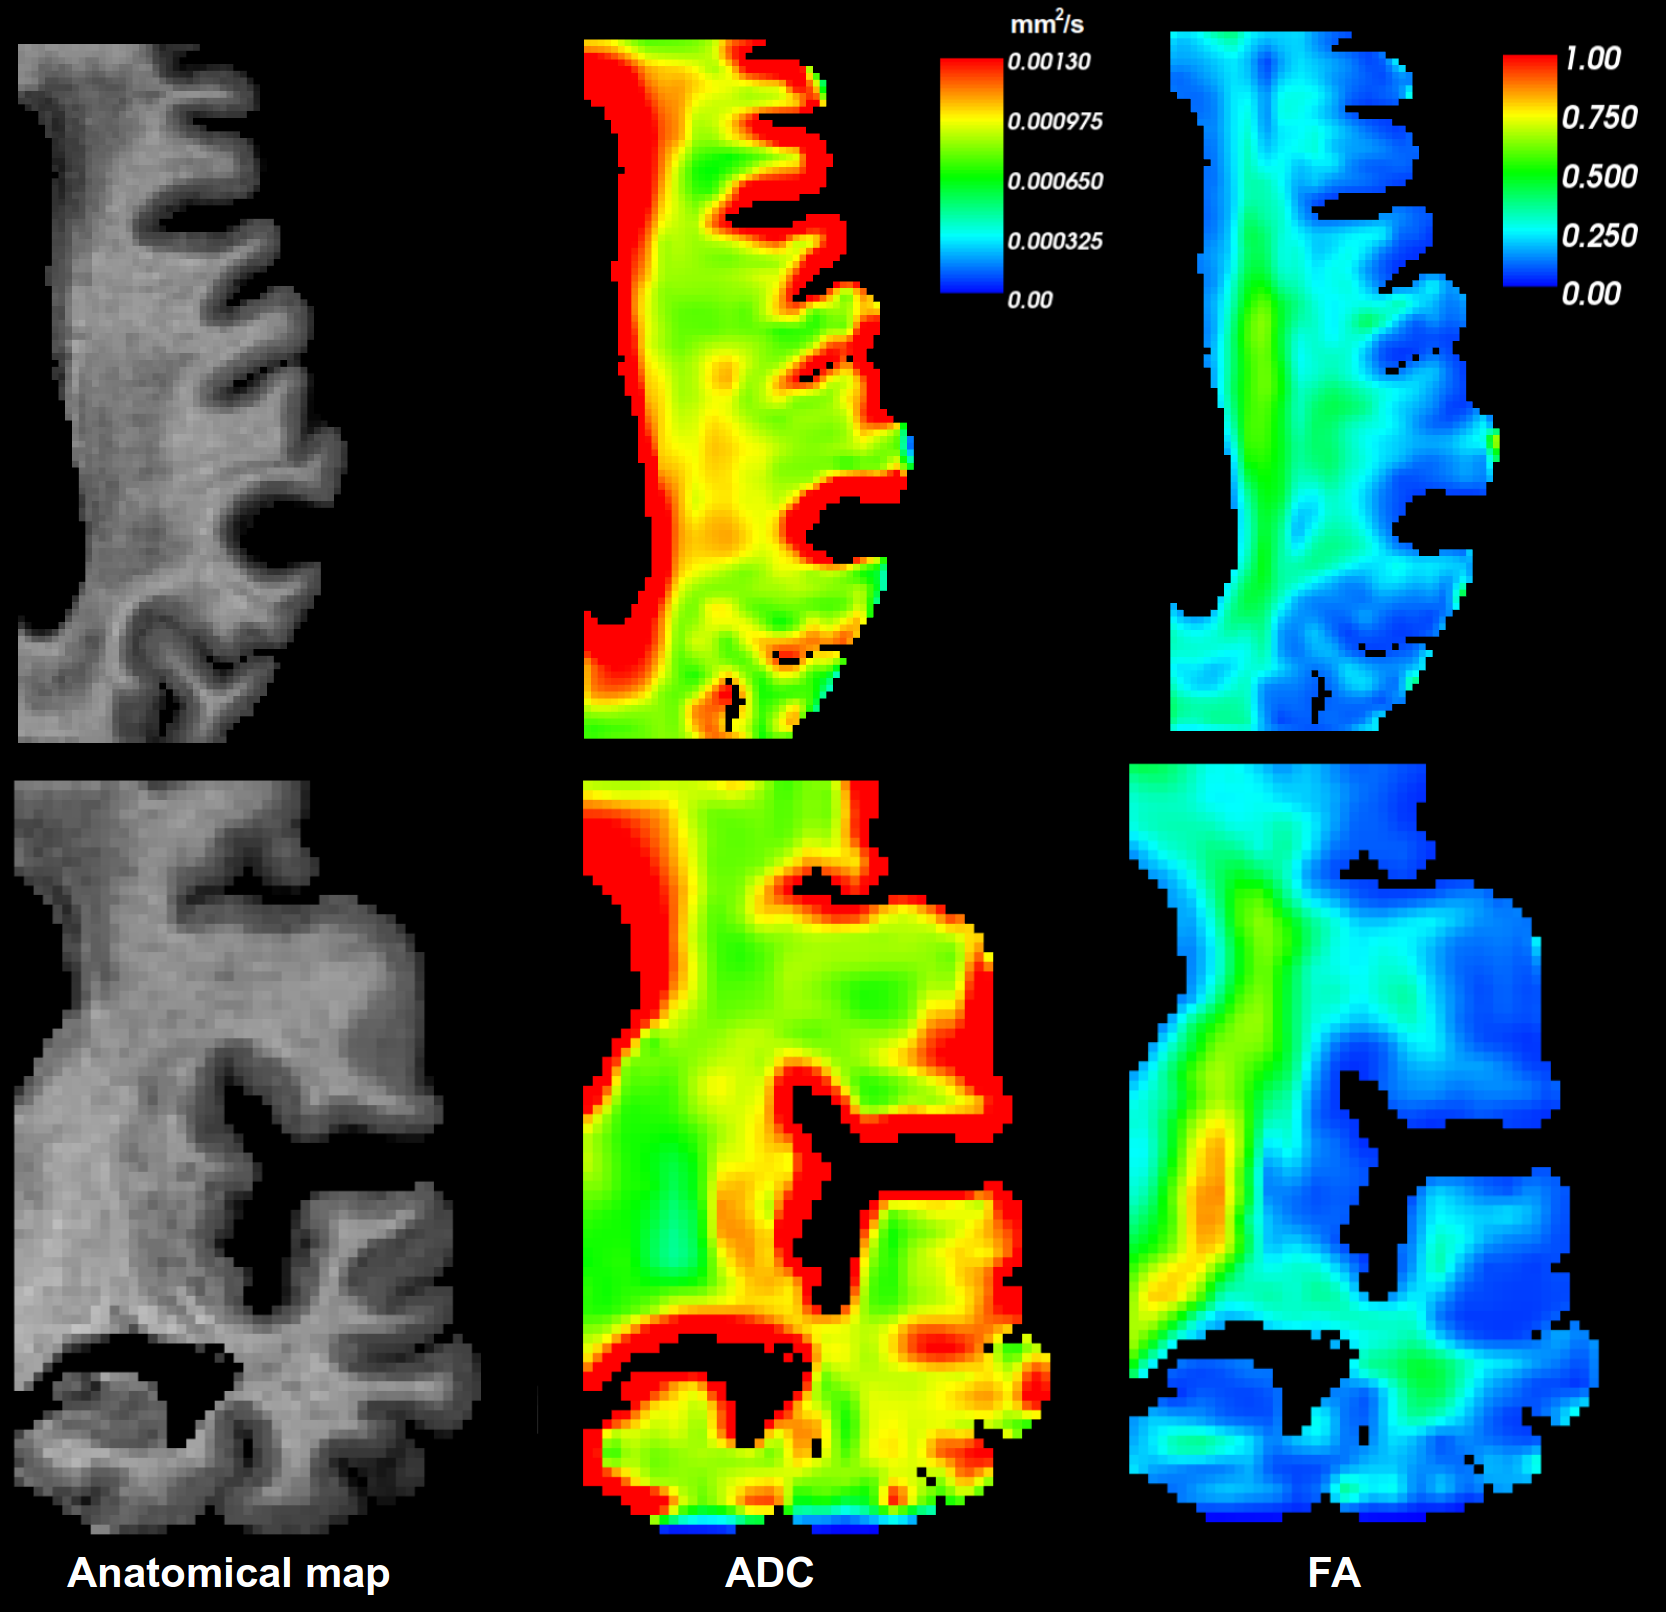
\includegraphics[width=0.80\textwidth]{DTI-zoom.png} 
\label{FIG::DTI} 
\caption{The left panel show the anatomical map. The middle panel show the apparent diffusion coefficients (ADC) obtained from DTI. The right panel shows the computed fractional anisotropy (FA) from the DTI.}
\end{figure}







\subsection{PDE constrained optimization algorithm} 

\kam{
Noen detaljer her om element methode, optimerings algoritme, prekondisjonering
grid, osv. 
}




\subsection*{Manufactured Solution}
In order to verify our strategy and test the dependency of the
regularization paramters, we perform a test case with a
known solution.  
The manufactured observations was obtained by forward computation of Eq.\ref{Eq::PDE} with the Dirichlet boundary condition defined as
\begin{equation}
g(t)_{\partial \Omega_1} = 0.3 +0.167t - 0.007t\sp{2} \qquad  0 \leq t \leq 24.
\label{EQ::DIRI}
\end{equation}
The timestep was $dt = 0.02$, and the diffusion coefficients were selected to be 
\begin{equation}
D_{\Omega_1} = 1000 \quad , \quad D_{\Omega_2} = 4.0 \quad , \quad D_{\Omega_3} = 8.0 
\end{equation}  
The magnitude order for $\quad D_{\Omega_2} $ and $\quad D_{\Omega_2}$ were chosen to resemble diffusion coefficient for water in grey and white matter, but the relation between the coeffieicents were not preserved. The diffusion coefficent in the csf was chosen given [cite Bryne and Kent]. The manufactured forward computation gave a total of 120 possible observation time points. These points will be denoted as $t_i$.

The mesh construction was patient-specific and was constructed by using the MRI of a patient diagnosed with idiopathic normal pressure hydrocephalus (iNPH). The software Freesurfer was used in segmentation and creating the polyhedral surfaces of the white and grey matter. Then the use of T2 weighted MRI was used to segment the CSF compartment surrounding the cerebral and the lateral ventricles. The module BrainMesh (currently in testing) (BrainMesh code accessibility {\color{red} kan ta med eller bare si CGAL}) CGAL \cite{cgal:rty-m3-18b} was used to combine the polyhedral surfaces and to construed the mesh. The computational requirement for the resulting mesh was significant, therefore two submesh was also constructed, see Fig.\ref{Fig::Mesh}.
\begin{figure}
\centering
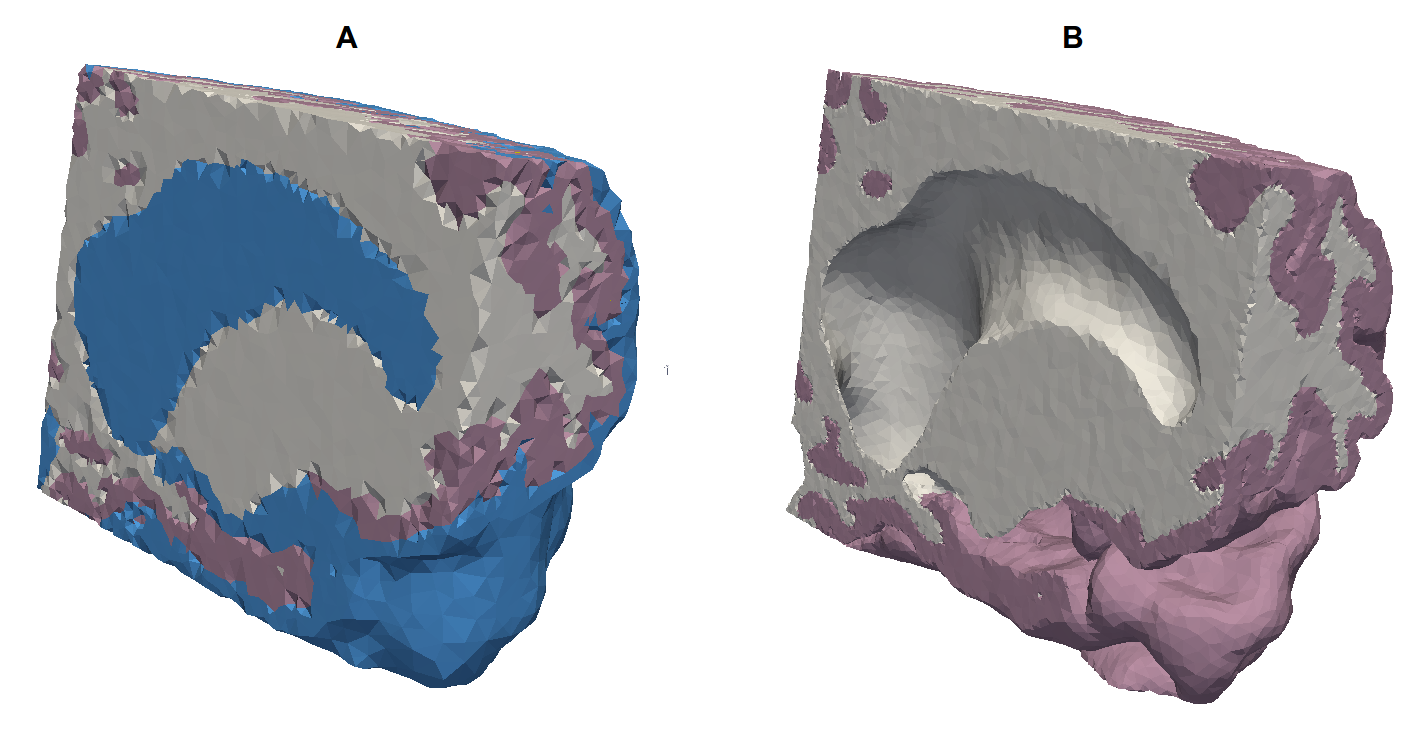
\includegraphics[scale=0.2]{mesh.png} 
\label{figmesh} 
\caption{A) Shows the mesh created from the baseline MR image with 3 domains. B) Shows the mesh created from the baseline MR image with 2 domains.  }
\label{Fig::Mesh}
\end{figure}
The 3 domain mesh in Fig.\ref{Fig::Mesh} A, consists of 244318 tetrahedral cells and 22057 vertices, while the 2 domain mesh Fig.\ref{Fig::Mesh} B consists of 335589 tetrahedral cells and 73002 vertices. The dimension of the mesh coordiantes are $\mathrm{mm}$.




\section{Results}
Below we will discuss the parameter identification and its sensitivity with respect to regularization parameters, noise and time-resolution. 
In presentation of the results, the relative error norm  $||\cdot||_{RE}$ is defined as 
\begin{equation}
|| X ||_{RE} = \frac{X_{found} -X_{true} }{ X_{true} }
\end{equation}
with $X$ as an arbitrary scalar control parameter. For the boundary parameter $g$, the relative error norm is defined as 
\begin{equation}
|| g ||_{RE} = \frac{ \sum\limits_t\sp{k}||| g_{found}(t) -g_{true}(t)||_{L(\Omega_1)} }{  \sum\limits_t\sp{k}||g_{true}(t)||_{L(\Omega_1)} }
\end{equation}
In the case that the minimization algorithm fails to converge within 1000 iteration will be indicated by a hyphen.  

\subsection{The relaxation parameters}
To assess the sensitivity of the the objective functional defined in Eq.\ref{Eq::F} with respect to the regularization parameters $\alpha$ and $\beta$ 
we perform a systematic study of the reconstruction of the manufactured solution with respect to a wide range of regularization parameters. 
Ideally, the approach should have a wide range of parameters in which the reconstruction algorithm yields very similar end-results although
the convergence may vary substatantially.
 The evaluation of different regularization parameters was done by solving the optimization with different values of $\alpha$ and $\beta$ and compare the controls with the manufactured solution. The observation times were selected with $t_i \in  \lbrace$ 2.4, 4.8, 7.2, 9.6, 12.0, 14.4, 16.8, 19.2, 21.6, 24.0 $\rbrace$, and the number of time-steps in the forward problem was set to $k= 10$. 

The results are shown in Tabel~\ref{Tab::1} together with the number of iteration used to reach the convergence criteria. For $\alpha= 1.0$, it can be observed that there is a significant relative error for $D_{\Omega_1}$. The other control parameters also show an increased relative error when compared to other values of $\alpha$. 

\begin{figure}
\centering
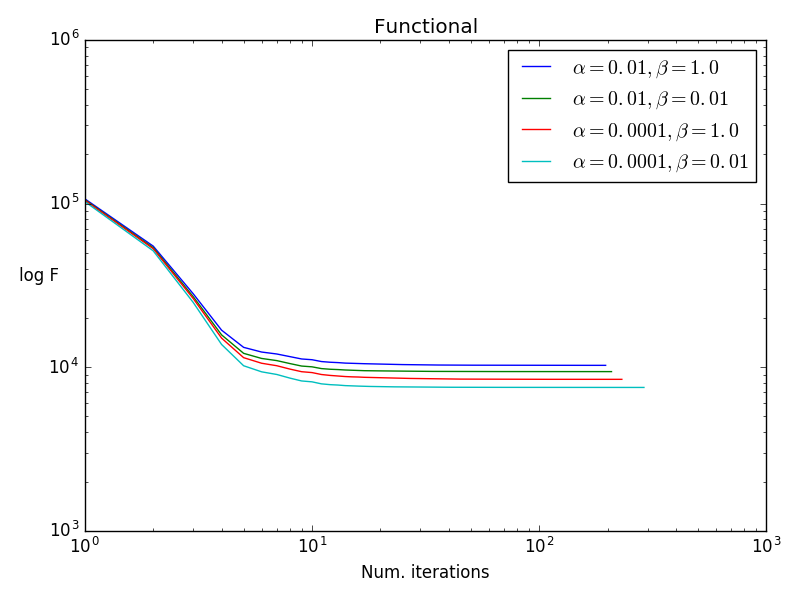
\includegraphics[scale=0.2]{convergence_0}  
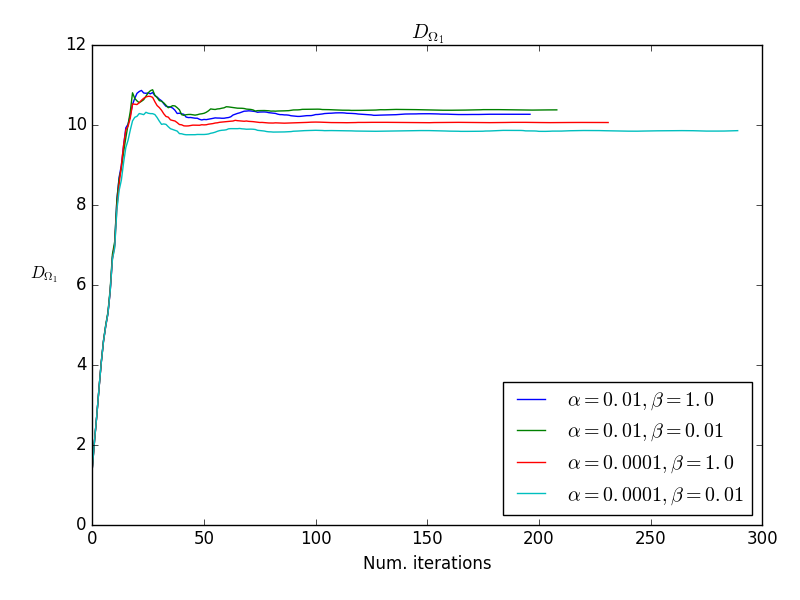
\includegraphics[scale=0.2]{convergence_1}  
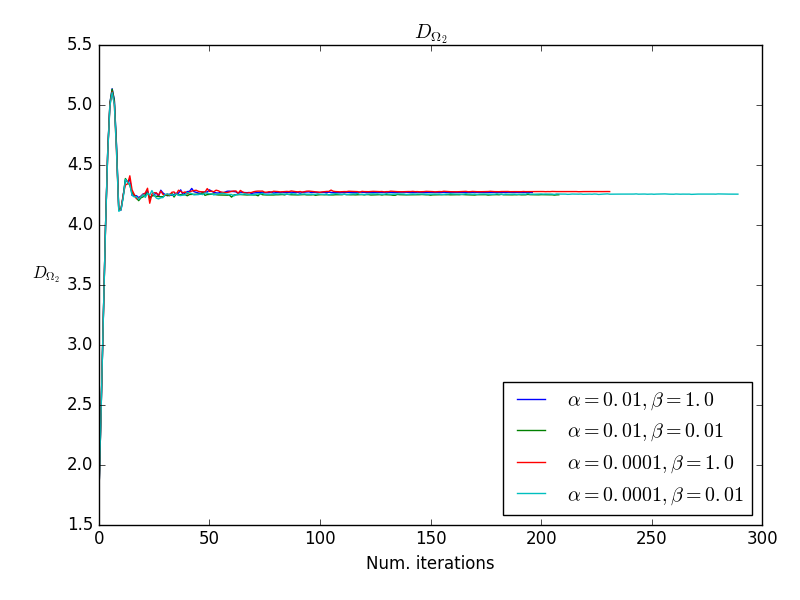
\includegraphics[scale=0.2]{convergence_2}  
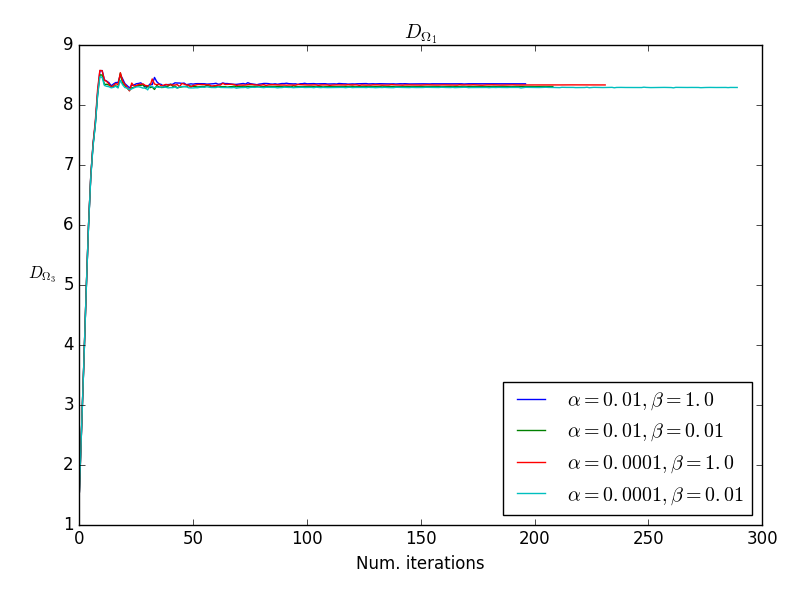
\includegraphics[scale=0.2]{convergence_3}  
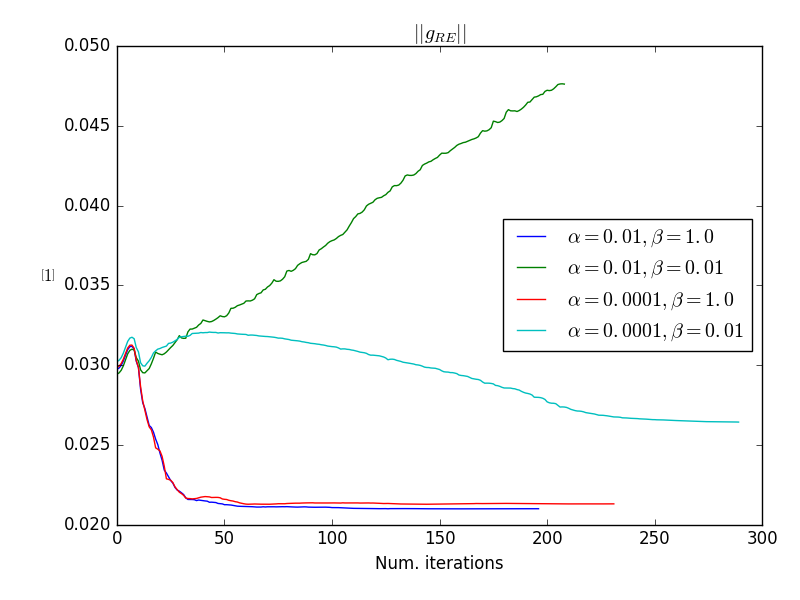
\includegraphics[scale=0.2]{convergence_4}  
\label{convergence}
\caption{Convergence of the diffusion coefficients, boundary conditions and functional with respect to different $\alpha$ and $\beta$ values. } 
\end{figure}



\subsection{The noise susceptibility}
The MRI data contains noise, hence an investigation to the noise susceptibility is needed. This was done by adding uniform noise in the range $\lbrace -n_{amp} , n_{amp} \rbrace $, with $n_{amp}$ defined as noise amplitude, to the manufactured observations. Then the optimization was solved by varying the regularization parameters $\alpha$ and $\beta$. Figure~\ref{12hourswithnoise} and Figure~\ref{24hourswithnoise} show the reconstruction of the manufactured solution with 
different noise levels with $\alpha=0.0001$ and $\beta=1.0$. Clearly, the reconstruction shown in the lower rows is quite robust with respect to the various levels
of noise shown in the upper rows.      

In Tabel~\ref{Tab::Noise0.03}, we can see that a noise amplitude of 0.03, (10$\%$ of maximum initial condition) had negligible effect on the relative error. However, in Tabel~\ref{Tab::Noise0.3} the noise amplitude was increased to 0.3 (100$\%$ of maximum initial condition) and it is observed that for  $\alpha < 1.0e-3$  $\beta < 1.0e-3$ the optimization failed to converge before reaching maximum iteration of 1000 steps. Furthermore, the relative boundary error $||g||_{RE(\Omega)}$ is  larger for lower values of $\beta$. 

\begin{figure}
\centering
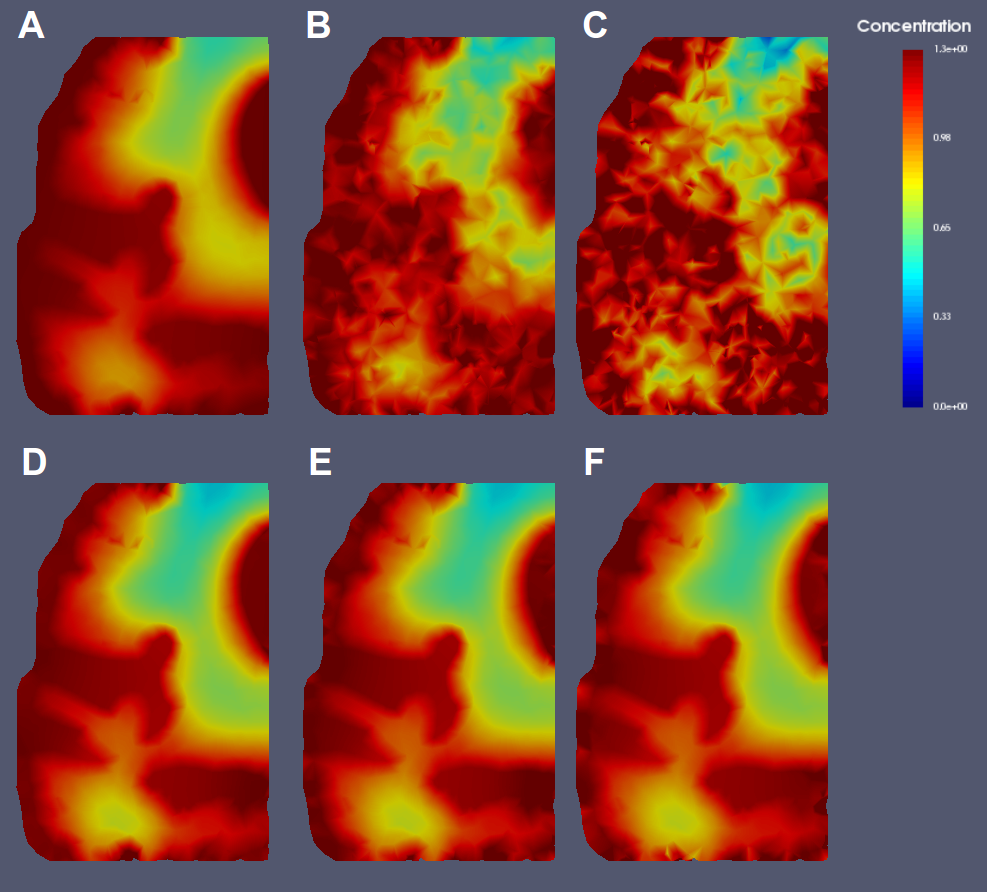
\includegraphics[scale=0.4]{27-12-hours-scale-0-1-3.png}  
\caption{The upper row shows the manufactured observation, A ) Shows the manufactured observation at time-point 24 with no noise added. B) Shows the manufactured observation at time-point 24 with an noise amplitude of 0.15. C)Shows the manufactures observation at time-point 24 with noise amplitude of 0.3. The lower row shows the results with optimized parameter obtained with $\alpha=0.0001$, $\beta=1.0$ and $k=27$. D) Shows the resulting state given the observation in A. E)  Shows the resulting state given the observation in B .F) Shows the resulting state given the observation in C. }
\label{12hourswithnoise}
\end{figure}


\begin{figure}
\centering
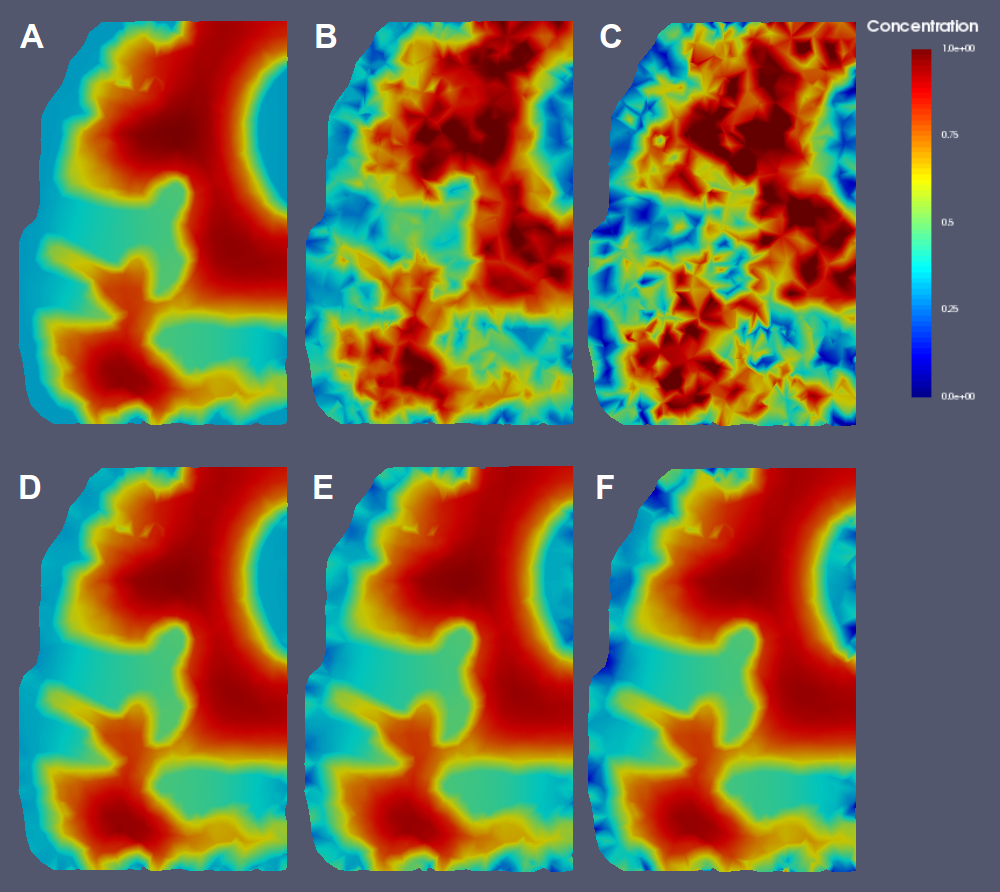
\includegraphics[scale=0.4]{27-24-hours-scale-0-1.png}
\caption{The upper row shows the manufactured observation, A ) Shows the manufactured observation at time-point 24 with no noise added. B) Shows the manufactured observation at time-point 24 with a noise amplitude of 0.15. C)Shows the manufactures observation at time-point 24 with noise amplitude of 0.3. The lower row shows the results with optimized parameter obtained with $\alpha=0.0001$, $\beta=1.0$ and $k=27$. D) Shows the resulting state given the observation in A. E)  Shows the resulting state given the observation in B .F) Shows the resulting state given the observation in C.  }
\label{24hourswithnoise}
\end{figure}


\subsection{The number of timessteps}
Increasing the number of timesteps in the simulations potentially allow for a more accurate temporal reconstruction, but at the same time the number of observations per control decreases and the regularization therefore may play a larger role. Furthermore,  the computational cost for each iteration of the L-BFGS-B algorithm as one
forward solve is performed per iteration. Thus finding the number of timesteps for an effective convergence can help for larger meshes. The computation vary the timesteps with 10, 20 and 40 timesteps. Additionally, the computation will use a few variations of the regularization parameters that gives small relative errors. 

This gave the values presented in Tab.\ref{TAB::timesteps}, and can be seen that increase in the number of timesteps causes a decrease in the relative error. 

\subsection{The number of observations}
The dependency on observations is relevant, since the number of observations of the MRI data is limited. This was investigated by changing the number of observations, and examine the resulting states. The number of observation were chosen to be 5, 10  and 20, and times were set to be evenly spaced. 

The results are shown in Tab.\ref{TAB::timesteps}, Tab.\ref{TAB::double} and Tab.\ref{TAB::half}. In the case of 10 observations, the number of timesteps showed a decrease in the relative error. Similar effects was observed for 5 and 20 observations. However, the variation of observations did not show a consistent decrease in error. And the variation in the relative error indicates oscillations in the convergence. 

\subsection{Sparse observations}
The MRI data contains observations after the injection of CSF tracer. These observation are unevenly distributed in time resulting in large time intervals with no observations. Therefore the effect of these temporal gaps in the observations will be evaluated. This was done by selecting the observation times as follows  $t_i = \lbrace$0.8, 1.0, 1.2, 1.8, 2.4, 3.6, 5.4, 7.6, 24.0$\rbrace$. The regularization parameters was selected, so that the error would be minimized,and noise was also added.

The results are shown in Tab.\ref{Tab::Hole1} and Tab\ref{Tab::Hole2}, and it can be observed that the addition of noise caused $\beta=1.0$ to converge the same. Comparing the values in Tab\ref{Tab::Hole1} and Tab.\ref{TAB::timesteps}, showed that the relative error increased.  

\subsection{MRI Data} 
The MRI data consisted of the observations at times $t_i \in \lbrace$ 0.00, 0.16, 0.39, 0.55, 0.77, 2.09, 6.05, 24.06, 47.84, 698.02 $\rbrace (hours)$ with the time $t_i=0.00$ as the observation 1-2 hours after the tracer was injected. There was no significant visible change in the tracer between the observations at $\lbrace $ 0.00, 0.16, 0.39, 0.55, 0.77 $ \rbrace$. This prompted the use of the following observation times  $0.00, 2.09, 6.05, 24.06, 47.84$. 

The estimation of tracer concentration proved difficult in the CSF compartment. Therefore the 2 domain mesh, shown in Fig.\ref{figmesh} was used in the computation. The boundary control was set to the external boundary of both domains, and the subscript in $D_w$ and $D_g$ denotes white and grey diffusion coefficients. Furthermore, bounds were added to the L-BFGS-B algorithm to ensure non-negative boundary controls and the convergence criteria was adjusted to $gtol=6.0e-1$. 

The results are shown in Tab.\ref{Tab::Real-data}, 
and the observation together with resulting states are displayed in Fig.\ref{Fig::realdata}


 

\subsection*{DTI comparison}
The median diffusion coefficient in the DTI was estimated to be 8.7e-4 $\mathrm{mm\sp{2}/s}$ in   white matter and 1.0e-3 $\mathrm{mm\sp{2}/s}$ in grey matter.   %This corresponds to 3.1 $\mathrm{mm\sp{2}/h}$ and  3.6 $\mathrm{mm\sp{2}/h}$. 
The self-diffusivity of water have been estimated to be around 3.0e-3$\mathrm{mm\sp{2}/s}$ for  $37\sp{o}C$.% This corresponds to 10.8 $\mathrm{mm\sp{2}/h}$ and  $\mathrm{mm\sp{2}/h}$. 

The reference value for Gd-DPTA was set to 3.8e-4 $\mathrm{mm\sp{2}/s}$. The values in Tab.\ref{Tab::Real-data} gives the value-range $1.5e-4 -2.7e-4\mathrm{mm\sp{2}/s}$ for the grey diffusion coefficient and  $2.2e-4 - 3.3e-4\mathrm{mm\sp{2}/s}$ for the white diffusion coefficient. These values are $20 -110 \%$ larger than the expected values for $D_{g}$,  and $100 - 200 \%$ larger than the expected values for $D_{w}$. 

The estimation assumes that the tortousity is independent on molecular size.

%The region with high diffusivity in the white matter, shown in Fig\ref{FIG::DTI}, gives a upper bound on the diffusion coefficient to be 1.3 $\mathrm{mm\sp{2}/s}$. 



%
% \begin{table}
%\centering
%\caption{Viser omgjøringer,estiamering og prosentvis forskjell for min og max control/optimerte verdier . Unit $\left[ \mathrm{mm\sp{2}/h} \right]$}
%\resizebox{\textwidth}{!}{\begin{tabular}{*{6}c}
%$ D\sp{free}_{water} $ & $ D\sp{DTI}__{g} $ & $ D\sp{DTI}_{w} $ & $D\sp{fre}__{Gd-DPTA} $ & $D\sp{ADC}__{g} $ & $ D\sp{ADC}_{w} $ & $ D\sp{ADC}_{g} -D\sp{OPT}_{g} $ &$ D\sp{ADC}_{w} -D\sp{OPT}_{w} $ \\
%\hline
%10.8 & 3.64 & 3.13 & 1.37 & 0.46 & 0.40 &  20 - 114 $\%$  & 100- 200 $\%$
%  -   &  -    & 4.86 &  - &  -   & 0.61 &   -                  &   0 - 100 $\%$       
%\end{tabular}} 
%\label{}
%\end{table} 
% 


{\color{red} tortuoisty mindre for støre molekyler ? }
%The region with high diffusivity in the white matter, shown in Fig\ref{FIG::DTI}, gives a upper bound on the diffusion coefficient to be 1.3 $\mathrm{mm\sp{2}/s}$

\section{Discussion}


\subsection{Manufactures Solution}
%The results from the manufactured solutions showed a robust method to compute diffusion coefficients. However, the maufactured solutions were constructed .. ? .. .
The computational model assumes isotropic diffusivity, but the anisotropy in the white matter is well documented, as shown by the FA in Fig\ref{FIG::DTI}. The region with high FA, can also be observed in the observation after 48 hours, shown in Fig.\ref{Fig::realdata}. This observation is after 48 hours, and the amount of tracer inside the anisotropic region is negligible. Therefore it would seem that the anisotropy do not have direct impact on the computations, since the computation can not evaluate a static environment. Thus observation of tracer in anisotropic regions are needed for the integration of anisotropy into the model. 
  
A more important factor are regions with higher diffusivity. Comparing Fig.\ref{FIG::DTI} and Fig \ref{Fig::realdata}, it can be observed that the region with high diffusivity also have a high tracer concentration. 

The computational model have 2 global controls for the diffusion coefficients, while it can be seen in  Fig.\ref{FIG::DTI} that diffusion coefficients can be considered a spacial function. Although the implmentaion of spacial control parameters are possible, it would siginificantly increase the computational cost. 

The coputational cost dependes on the relaxation parameteres, the number of controls and solution of the PDE.

   
  
It can also be taken into consideration to model the diffusion coefficients as a function in time, given the report of an increase clearance in rodents during sleeping [insert citation]. This follows the assumption that the clearance is related to diffusion, which means an increase in diffusivity. Since the properties of the tracer molecule do not change, this would mean that the tortuosity decreased and followed by an incearse in the ADC.

In Tab.\ref{Tab::Real-data}, it is shown that the grey matter diffusion coefficient have a consistent increase based on the decrease in the relaxation parameter $\beta$. This can be caused by the boundary control $g$, which exists along the entire boundary of the grey matter. Considering the that the grey matter volume has a depth less than 3 mm makes it susceptible to changes in $g$. This can be observed in the reconstruction in Fig.\ref{12hourswithnoise} and Fig.\ref{24hourswithnoise}, where the nosie is present at the boundary. 
  
  

A possible solution is to include the CSF compartment, but only use the observation in the white and grey matter. 




The hypothesis of the glymphatic system [insert citation] states that the waste is cleared through the veins in the cerebral. This gives the tracer an additional pathway that is not considered in the computational. The additional pathway can be modeled as a drainage, which can be included in the model as a sink source. This sink term can be added to the model as a control. 




 
\section{Conclusion}



%\begin{figure}
%\centering
%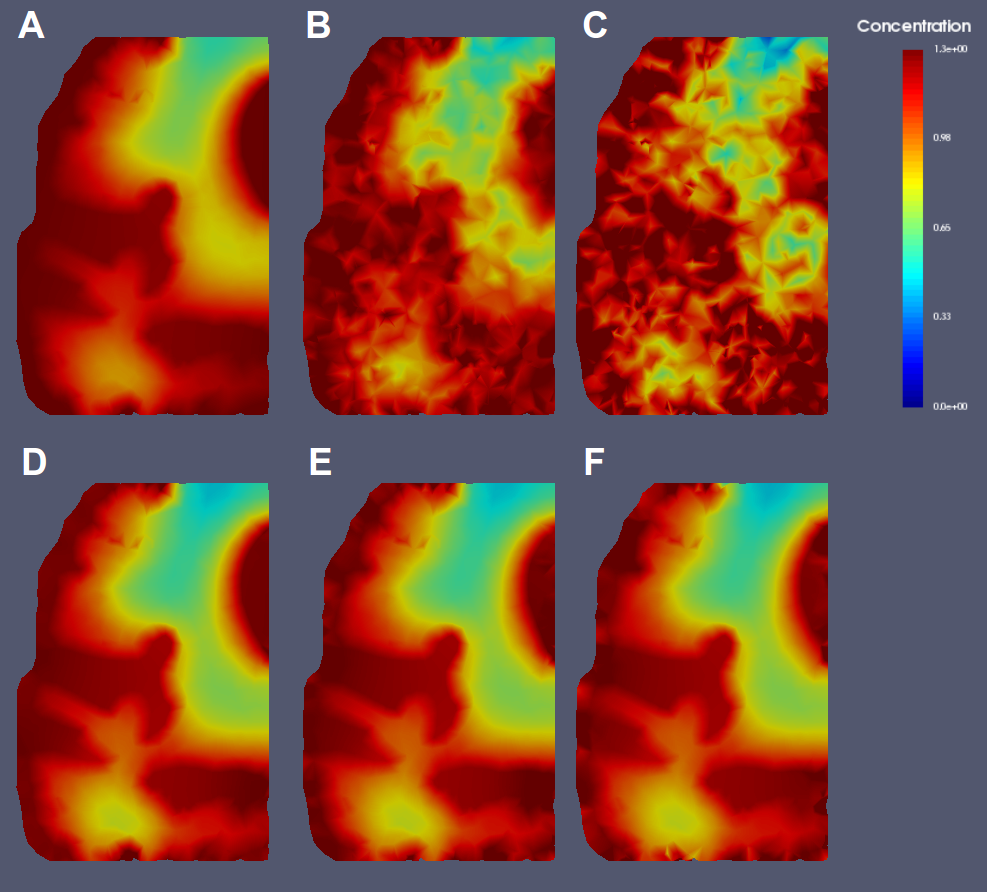
\includegraphics[scale=0.4]{27-12-hours-scale-0-1-3.png}  
%\caption{The upper row shows the manufactured observation, A ) Shows the manufactured observation at time-point 24 with no noise added. B) Shows the manufactured observation at time-point 24 with an noise amplitude of 0.15. C)Shows the manufactures observation at time-point 24 with noise amplitude of 0.3. The lower row shows the results with optimized parameter obtained with $alpha=0.0001$, $\beta=1.0$ and $k=27$. D) Shows the resulting state given the observation in A. E)  Shows the resulting state given the observation in B .F) Shows the resulting state given the observation in C. }
%\end{figure}
%
%
%\begin{figure}
%\centering
%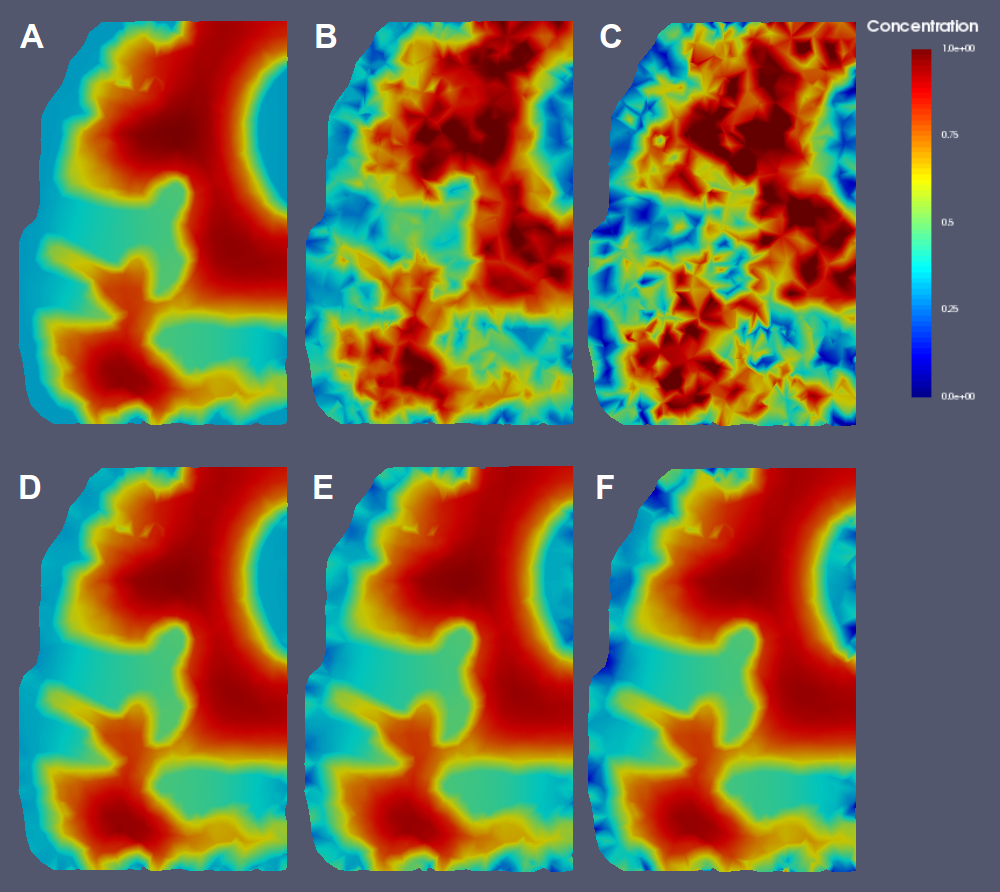
\includegraphics[scale=0.4]{27-24-hours-scale-0-1.png}
%\caption{The upper row shows the manufactured observation, A ) Shows the manufactured observation at time-point 24 with no noise added. B) Shows the manufactured observation at time-point 24 with a noise amplitude of 0.15 {\color{red} explain noise ampliutde}. C)Shows the manufactures observation at time-point 24 with noise amplitude of 0.3. The lower row shows the results with optimized parameter obtained with $alpha=0.0001$, $\beta=1.0$ and $k=27$. D) Shows the resulting state given the observation in A. E)  Shows the resulting state given the observation in B .F) Shows the resulting state given the observation in C.  }
%\end{figure}
% 
% 
% 
%
% 


\bibliographystyle{amsplain}
\bibliography{references}


\newpage 
\newgeometry{top=0.5cm}




 
 
 



 
\begin{figure}
\centering
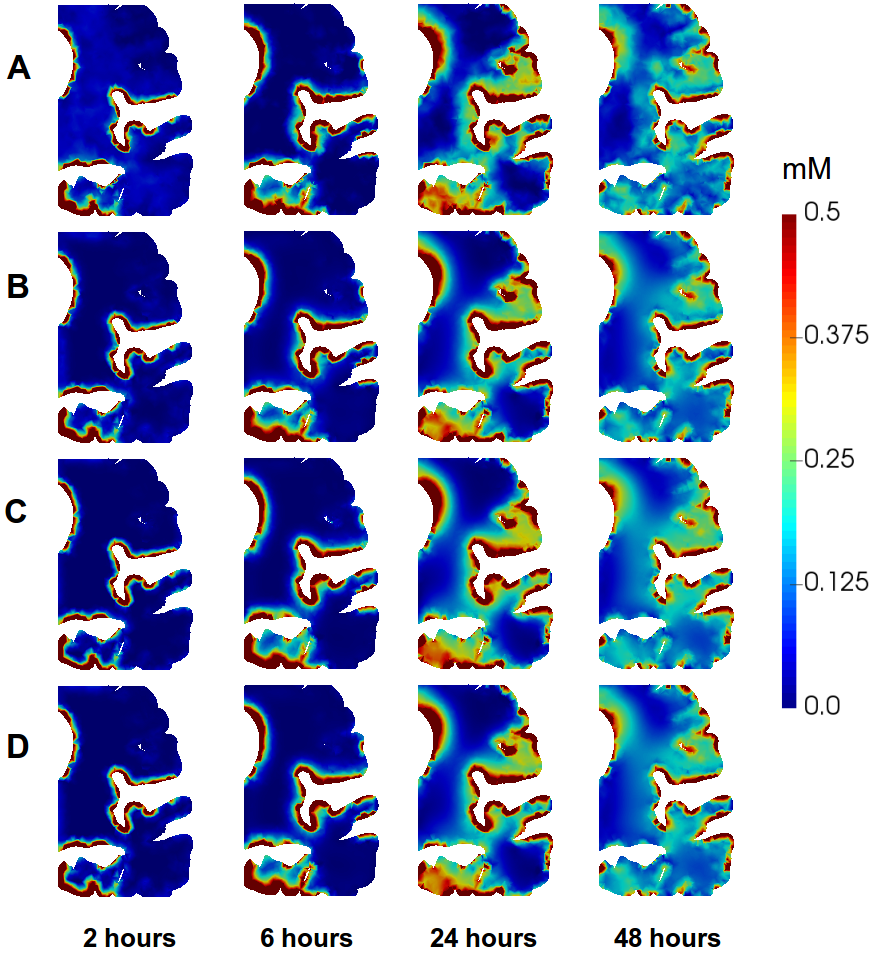
\includegraphics[width=0.95\textwidth]{different.png} 
\caption{Row A) shows the observation at times 2 hours, 6 hours, 24 hours and 48 hours after the first observation with tracer. Row B) shows the corresponding states with the relaxation parameters set to $ \alpha=0.01$ and $\beta=0.01$.   Row C) shows the corresponding states with the relaxation parameters set to $ \alpha=0.0001$ and $\beta=1.0$.
 Row D) shows the corresponding states with the relaxation parameters set to$ \alpha=1.0e-6$ and $\beta=0.1$. The color-bar was restricted to the range $ \lbrace 0 ,0.5 \rbrace$. }
\label{Fig::realdata}
\end{figure}

\begin{table}
\centering
\caption{Shows the regularization parameters $\alpha$ and $\beta$, number of timesteps $k$ and number of observation $\tau$ with the resulting number of iterations and the relative error for the control parameters. }
\resizebox{0.9\textwidth}{!}{\begin{tabular}{*{8}c}
$\alpha$ & $\beta$ & k  & iter & $ ||D_{\Omega_1}||_{RE}$ & $ ||D_{\Omega_2}||_{RE} $ & $||D_{\Omega_3}||_{RE}$ & $||g||_{RE}$ \\
\hline
  1.0e+00 	 & 1.0e+00 	 & 10 & 225 	 & +4.148 & +0.304 & +0.092 & +0.135 \\ 
%\rowcolor{red}  1.0e+00 	 & 1.0e-01 	 & 10 & 206 	 & +4.272 & +0.305 & +0.091 & +0.142 \\ 
 1.0e+00 	 & 1.0e-02 	 & 10 & 233 	 & +4.272 & +0.305 & +0.091 & +0.143 \\ 
%\rowcolor{red}  1.0e+00 	 & 1.0e-03 	 & 10 & 208 	 & +4.437 & +0.305 & +0.091 & +0.143 \\ 
 1.0e+00 	 & 1.0e-04 	 & 10 & 204 	 & +4.271 & +0.306 & +0.091 & +0.143 \\ 
%\rowcolor{red}  1.0e+00 	 & 1.0e-05 	 & 10 & 203 	 & +4.400 & +0.305 & +0.091 & +0.143 \\ 
 1.0e+00 	 & 1.0e-06 	 & 10 & 222 	 & +4.584 & +0.304 & +0.090 & +0.143 \\
 
% 1.0e-01 	 & 1.0e+00 	 & 10 & 207 	 & +0.127 & +0.093 & +0.041 & +0.027 \\ 
 %1.0e-01 	 & 1.0e-01 	 & 10 & 196 	 & +0.121 & +0.093 & +0.041 & +0.046 \\ 
% 1.0e-01 	 & 1.0e-02 	 & 10 & 232 	 & +0.123 & +0.093 & +0.041 & +0.056 \\ 
 %1.0e-01 	 & 1.0e-03 	 & 10 & 183 	 & +0.122 & +0.093 & +0.040 & +0.057 \\ 
% 1.0e-01 	 & 1.0e-04 	 & 10 & 212 	 & +0.122 & +0.093 & +0.040 & +0.057 \\ 
 %1.0e-01 	 & 1.0e-05 	 & 10 & 168 	 & +0.122 & +0.093 & +0.041 & +0.057 \\
% 1.0e-01 	 & 1.0e-06 	 & 10 & 195 	 & +0.122 & +0.093 & +0.041 & +0.057 \\ 

 1.0e-02 	 & 1.0e+00 	 & 10 & 227 	 & +0.015 & +0.067 & +0.039 & +0.018 \\ 
 %1.0e-02 	 & 1.0e-01 	 & 10 & 153 	 & +0.006 & +0.065 & +0.039 & +0.021 \\ 
 1.0e-02 	 & 1.0e-02 	 & 10 & 184 	 & +0.005 & +0.065 & +0.039 & +0.039 \\ 
 %1.0e-02 	 & 1.0e-03 	 & 10 & 176 	 & +0.004 & +0.065 & +0.039 & +0.048 \\ 
 1.0e-02 	 & 1.0e-04 	 & 10 & 195 	 & +0.005 & +0.065 & +0.039 & +0.049 \\ 
 %1.0e-02 	 & 1.0e-05 	 & 10 & 215 	 & +0.004 & +0.065 & +0.039 & +0.051 \\ 
 1.0e-02 	 & 1.0e-06 	 & 10 & 205 	 & +0.005 & +0.065 & +0.039 & +0.050 \\ 

 %1.0e-03 	 & 1.0e+00 	 & 10 & 179 	 & +0.004 & +0.064 & +0.039 & +0.019 \\ 
 %1.0e-03 	 & 1.0e-01 	 & 10 & 221 	 & -0.005 & +0.063 & +0.039 & +0.018 \\ 
 %1.0e-03 	 & 1.0e-02 	 & 10 & 89 	 & -0.007 & +0.063 & +0.039 & +0.026 \\ 
 %1.0e-03 	 & 1.0e-03 	 & 10 & 77 	 & -0.005 & +0.062 & +0.039 & +0.027 \\ 
 %1.0e-03 	 & 1.0e-04 	 & 10 & 100 	 & -0.006 & +0.062 & +0.039 & +0.027 \\ 
 %1.0e-03 	 & 1.0e-05 	 & 10 & 105 	 & -0.006 & +0.062 & +0.039 & +0.027 \\ 
 %1.0e-03 	 & 1.0e-06 	 & 10 & 123 	 & -0.007 & +0.062 & +0.039 & +0.028 \\ 


 1.0e-04 	 & 1.0e+00 	 & 10 & 236 	 & +0.004 & +0.063 & +0.039 & +0.019 \\ 
 %1.0e-04 	 & 1.0e-01 	 & 10 & 195 	 & -0.006 & +0.062 & +0.039 & +0.018 \\ 
 1.0e-04 	 & 1.0e-02 	 & 10 & 152 	 & -0.006 & +0.062 & +0.039 & +0.022 \\ 
 %1.0e-04 	 & 1.0e-03 	 & 10 & 119 	 & -0.008 & +0.062 & +0.039 & +0.026 \\ 
 1.0e-04 	 & 1.0e-04 	 & 10 & 106 	 & -0.007 & +0.062 & +0.039 & +0.026 \\ 
 %1.0e-04 	 & 1.0e-05 	 & 10 & 109 	 & -0.007 & +0.062 & +0.039 & +0.026 \\ 
 1.0e-04 	 & 1.0e-06 	 & 10 & 99 	 & -0.008 & +0.062 & +0.039 & +0.026 \\
 
 %1.0e-05 	 & 1.0e+00 	 & 10 & 139 	 & +0.004 & +0.063 & +0.039 & +0.019 \\ 
 %1.0e-05 	 & 1.0e-01 	 & 10 & 170 	 & -0.006 & +0.062 & +0.039 & +0.018 \\ 
 %1.0e-05 	 & 1.0e-02 	 & 10 & 182 	 & -0.007 & +0.062 & +0.039 & +0.020 \\ 
 %1.0e-05 	 & 1.0e-03 	 & 10 & 70 	 & -0.007 & +0.062 & +0.039 & +0.026 \\ 
 %1.0e-05 	 & 1.0e-04 	 & 10 & 77 	 & -0.007 & +0.062 & +0.039 & +0.026 \\ 
 %1.0e-05 	 & 1.0e-05 	 & 10 & 104 	 & -0.008 & +0.062 & +0.039 & +0.026 \\ 
 %1.0e-05 	 & 1.0e-06 	 & 10 & 92 	 & -0.007 & +0.062 & +0.039 & +0.026 \\ 

 1.0e-06 	 & 1.0e+00 	 & 10 & 163 	 & +0.003 & +0.064 & +0.039 & +0.019 \\ 
 %1.0e-06 	 & 1.0e-01 	 & 10 & 218 	 & -0.006 & +0.062 & +0.039 & +0.018 \\ 
 1.0e-06 	 & 1.0e-02 	 & 10 & 134 	 & -0.008 & +0.062 & +0.039 & +0.023 \\ 
 %1.0e-06 	 & 1.0e-03 	 & 10 & 79 	 & -0.006 & +0.062 & +0.039 & +0.026 \\ 
 1.0e-06 	 & 1.0e-04 	 & 10 & 107 	 & -0.007 & +0.062 & +0.039 & +0.026 \\ 
 %1.0e-06 	 & 1.0e-05 	 & 10 & 103 	 & -0.008 & +0.062 & +0.039 & +0.026 \\ 
 1.0e-06 	 & 1.0e-06 	 & 10 & 91 	 & -0.008 & +0.062 & +0.039 & +0.026 \\  
\end{tabular}}
\label{Tab::1}
\end{table} 







\newpage
\begin{table}
\centering
\caption{Shows the relaxation parameters $\alpha$ and $\beta$, number of timesteps $k$, the resulting number of iterations, the relative error of the estimated optimal parameters for the diffusion coefficients and the relative error for $g$. The noise amplitude was set to 0.03, and $ t_i=[2.4, 4.8, 7.2, 9.6, 12.0, 14.4, 16.8, 19.2, 21.6, 24.0]$ }
\resizebox{0.8\textwidth}{!}{\begin{tabular}{*{8}c}
$\alpha$ & $\beta$ & k  & iter & $ ||D_{\Omega_1}||_{RE} $ & $||D_{\Omega_2}||_{RE}$ & $||D_{\Omega_3}||_{RE}$ & $||g||_{RE}$\\
\hline
 1.0e+00 	 & 1.0e+00 	 & 10 & 218 	 & +4.266 & +0.304 & +0.092 & +0.135 \\ 
 %1.0e+00 	 & 1.0e-01 	 & 10 & 223 	 & +4.565 & +0.304 & +0.090 & +0.142 \\ 
 1.0e+00 	 & 1.0e-02 	 & 10 & 199 	 & +4.268 & +0.305 & +0.090 & +0.143 \\ 
% 1.0e+00 	 & 1.0e-03 	 & 10 & 222 	 & +4.274 & +0.305 & +0.090 & +0.143 \\ 
 1.0e+00 	 & 1.0e-04 	 & 10 & 211 	 & +4.448 & +0.306 & +0.090 & +0.143 \\ 
% 1.0e+00 	 & 1.0e-05 	 & 10 & 227 	 & +4.527 & +0.304 & +0.090 & +0.143 \\ 
 1.0e+00 	 & 1.0e-06 	 & 10 & 263 	 & +4.266 & +0.306 & +0.091 & +0.143 \\ 
 
 %1.0e-01 	 & 1.0e+00 	 & 10 & 167 	 & +0.131 & +0.093 & +0.041 & +0.027 \\ 
% 1.0e-01 	 & 1.0e-01 	 & 10 & 195 	 & +0.125 & +0.093 & +0.039 & +0.046 \\ 
% 1.0e-01 	 & 1.0e-02 	 & 10 & 218 	 & +0.126 & +0.093 & +0.040 & +0.056 \\ 
% 1.0e-01 	 & 1.0e-03 	 & 10 & 161 	 & +0.129 & +0.094 & +0.040 & +0.057 \\ 
% 1.0e-01 	 & 1.0e-04 	 & 10 & 180 	 & +0.135 & +0.092 & +0.042 & +0.057 \\ 
% 1.0e-01 	 & 1.0e-05 	 & 10 & 169 	 & +0.123 & +0.093 & +0.041 & +0.057 \\ 
% 1.0e-01 	 & 1.0e-06 	 & 10 & 201 	 & +0.119 & +0.093 & +0.040 & +0.057 \\ 

 1.0e-02 	 & 1.0e+00 	 & 10 & 183 	 & +0.013 & +0.067 & +0.040 & +0.018 \\ 
% 1.0e-02 	 & 1.0e-01 	 & 10 & 149 	 & +0.002 & +0.066 & +0.038 & +0.021 \\ 
 1.0e-02 	 & 1.0e-02 	 & 10 & 185 	 & -0.005 & +0.065 & +0.040 & +0.040 \\ 
% 1.0e-02 	 & 1.0e-03 	 & 10 & 213 	 & +0.004 & +0.066 & +0.038 & +0.049 \\ 
 1.0e-02 	 & 1.0e-04 	 & 10 & 151 	 & +0.008 & +0.066 & +0.039 & +0.047 \\ 
% 1.0e-02 	 & 1.0e-05 	 & 10 & 197 	 & +0.004 & +0.064 & +0.040 & +0.051 \\ 
 1.0e-02 	 & 1.0e-06 	 & 10 & 185 	 & +0.012 & +0.063 & +0.038 & +0.049 \\ 

% 1.0e-03 	 & 1.0e+00 	 & 10 & 183 	 & +0.007 & +0.062 & +0.038 & +0.019 \\ 
% 1.0e-03 	 & 1.0e-01 	 & 10 & 181 	 & -0.011 & +0.063 & +0.039 & +0.019 \\ 
% 1.0e-03 	 & 1.0e-02 	 & 10 & 122 	 & -0.008 & +0.063 & +0.040 & +0.025 \\ 
% 1.0e-03 	 & 1.0e-03 	 & 10 & 158 	 & -0.004 & +0.062 & +0.040 & +0.028 \\ 
% 1.0e-03 	 & 1.0e-04 	 & 10 & 168 	 & -0.013 & +0.063 & +0.038 & +0.029 \\ 
% 1.0e-03 	 & 1.0e-05 	 & 10 & 120 	 & -0.010 & +0.063 & +0.040 & +0.028 \\ 
% 1.0e-03 	 & 1.0e-06 	 & 10 & 132 	 & -0.002 & +0.062 & +0.039 & +0.028 \\ 

 1.0e-04 	 & 1.0e+00 	 & 10 & 176 	 & +0.000 & +0.063 & +0.039 & +0.019 \\ 
 %1.0e-04 	 & 1.0e-01 	 & 10 & 180 	 & -0.001 & +0.062 & +0.039 & +0.019 \\ 
 1.0e-04 	 & 1.0e-02 	 & 10 & 120 	 & +0.000 & +0.063 & +0.039 & +0.024 \\ 
 %1.0e-04 	 & 1.0e-03 	 & 10 & 119 	 & -0.004 & +0.062 & +0.039 & +0.026 \\ 
 1.0e-04 	 & 1.0e-04 	 & 10 & 77 	 & -0.005 & +0.061 & +0.038 & +0.027 \\ 
 %1.0e-04 	 & 1.0e-05 	 & 10 & 104 	 & -0.004 & +0.062 & +0.038 & +0.027 \\ 
 1.0e-04 	 & 1.0e-06 	 & 10 & 109 	 & -0.007 & +0.062 & +0.039 & +0.027 \\ 

 %1.0e-05 	 & 1.0e+00 	 & 10 & 220 	 & +0.005 & +0.063 & +0.039 & +0.019 \\ 
 %1.0e-05 	 & 1.0e-01 	 & 10 & 193 	 & -0.009 & +0.062 & +0.039 & +0.019 \\ 
 %1.0e-05 	 & 1.0e-02 	 & 10 & 163 	 & -0.013 & +0.063 & +0.039 & +0.021 \\ 
 %1.0e-05 	 & 1.0e-03 	 & 10 & 115 	 & -0.007 & +0.063 & +0.040 & +0.026 \\ 
 %1.0e-05 	 & 1.0e-04 	 & 10 & 82 	 & -0.007 & +0.062 & +0.038 & +0.027 \\ 
 %1.0e-05 	 & 1.0e-05 	 & 10 & 145 	 & -0.001 & +0.062 & +0.039 & +0.027 \\ 
 %1.0e-05 	 & 1.0e-06 	 & 10 & 147 	 & -0.012 & +0.061 & +0.040 & +0.027 \\ 

 1.0e-06 	 & 1.0e+00 	 & 10 & 138 	 & +0.002 & +0.063 & +0.039 & +0.019 \\ 
 %1.0e-06 	 & 1.0e-01 	 & 10 & 184 	 & -0.006 & +0.063 & +0.039 & +0.019 \\ 
 1.0e-06 	 & 1.0e-02 	 & 10 & 83 	 & -0.006 & +0.063 & +0.040 & +0.025 \\ 
 %1.0e-06 	 & 1.0e-03 	 & 10 & 91 	 & -0.013 & +0.063 & +0.039 & +0.026 \\ 
 1.0e-06 	 & 1.0e-04 	 & 10 & 109 	 & -0.005 & +0.062 & +0.038 & +0.027 \\ 
 %1.0e-06 	 & 1.0e-05 	 & 10 & 116 	 & -0.007 & +0.063 & +0.039 & +0.027 \\ 
 1.0e-06 	 & 1.0e-06 	 & 10 & 108 	 & +0.001 & +0.062 & +0.040 & +0.027 \\ 
\end{tabular}}
\label{Tab::Noise0.03}
\end{table} 
\begin{table}[t]
\centering
\caption{Shows the relaxation parameters $\alpha$ and $\beta$, number of timesteps $k$, the resulting number of iterations, the relative error of the estimated optimal parameters for the diffusion coefficients and the relative error for $g$. The noise amplitude was set to 0.3, and $t_i =[2.4, 4.8, 7.2, 9.6, 12.0, 14.4, 16.8, 19.2, 21.6, 24.0]$  }
\resizebox{0.8\textwidth}{!}{\begin{tabular}{*{8}c}
$\alpha$ & $\beta$ & k  & iter & $ ||D_{\Omega_1}||_{RE}$ & $||D_{\Omega_2}||_{RE} $ & $||D_{\Omega_3}||_{RE} $ & $||g||_{RE}$ \\
\hline
 1.0e+00 	 & 1.0e+00 	 & 10 & 212 	 & +4.268 & +0.310 & +0.073 & +0.138 \\ 
 %1.0e+00 	 & 1.0e-01 	 & 10 & 211 	 & +4.122 & +0.302 & +0.085 & +0.146 \\ 
 1.0e+00 	 & 1.0e-02 	 & 10 & 221 	 & +4.773 & +0.298 & +0.089 & +0.147 \\ 
 %1.0e+00 	 & 1.0e-03 	 & 10 & 257 	 & +4.872 & +0.301 & +0.090 & +0.147 \\ 
 1.0e+00 	 & 1.0e-04 	 & 10 & 238 	 & +4.186 & +0.293 & +0.097 & +0.148 \\ 
 %1.0e+00 	 & 1.0e-05 	 & 10 & 204 	 & +4.251 & +0.313 & +0.085 & +0.147 \\ 
 1.0e+00 	 & 1.0e-06 	 & 10 & 223 	 & +4.493 & +0.310 & +0.085 & +0.147 \\ 
 %1.0e-01 	 & 1.0e+00 	 & 10 & 145 	 & +0.126 & +0.100 & +0.054 & +0.035 \\ 
 %1.0e-01 	 & 1.0e-01 	 & 10 & 199 	 & +0.115 & +0.125 & +0.026 & +0.060 \\ 
 %1.0e-01 	 & 1.0e-02 	 & 10 & 217 	 & +0.128 & +0.092 & +0.036 & +0.071 \\ 
 %1.0e-01 	 & 1.0e-03 	 & 10 & 242 	 & +0.109 & +0.093 & +0.031 & +0.073 \\ 
 %1.0e-01 	 & 1.0e-04 	 & 10 & 275 	 & +0.187 & +0.094 & +0.028 & +0.073 \\ 
 %1.0e-01 	 & 1.0e-05 	 & 10 & 237 	 & +0.048 & +0.099 & +0.039 & +0.073 \\ 
 %1.0e-01 	 & 1.0e-06 	 & 10 & 225 	 & +0.092 & +0.111 & +0.055 & +0.073 \\ 
 1.0e-02 	 & 1.0e+00 	 & 10 & 208 	 & +0.017 & +0.075 & +0.037 & +0.029 \\ 
 %1.0e-02 	 & 1.0e-01 	 & 10 & 199 	 & -0.013 & +0.068 & +0.046 & +0.040 \\ 
 1.0e-02 	 & 1.0e-02 	 & 10 & 348 	 & -0.043 & +0.073 & +0.041 & +0.063 \\ 
% 1.0e-02 	 & 1.0e-03 	 & 10 & 400 	 & +0.056 & +0.058 & +0.031 & +0.075 \\ 
 1.0e-02 	 & 1.0e-04 	 & 10 & 393 	 & -0.050 & +0.088 & +0.044 & +0.077 \\ 
 %1.0e-02 	 & 1.0e-05 	 & 10 & 359 	 & +0.022 & +0.068 & +0.027 & +0.076 \\ 
 1.0e-02 	 & 1.0e-06 	 & 10 & 369 	 & +0.001 & +0.074 & +0.024 & +0.076 \\ 
 %1.0e-03 	 & 1.0e+00 	 & 10 & 207 	 & -0.001 & +0.065 & +0.051 & +0.029 \\ 
% 1.0e-03 	 & 1.0e-01 	 & 10 & 280 	 & +0.028 & +0.051 & +0.053 & +0.038 \\ 
 %1.0e-03 	 & 1.0e-02 	 & 10 & 565 	 & -0.059 & +0.076 & +0.033 & +0.053 \\ 
% 1.0e-03 	 & 1.0e-03 	 & 10 & 673 	 & -0.035 & +0.066 & +0.032 & +0.108 \\ 
 %\rowcolor{orange} 1.0e-03 	 & 1.0e-04 	 & 10 & 604 	 & -0.026 & +0.061 & +0.049 & +0.182 \\ 
 %1.0e-03 	 & 1.0e-05 	 & 10 & 666 	 & +0.012 & +0.070 & +0.038 & +0.182 \\ 
 %\rowcolor{orange} 1.0e-03 	 & 1.0e-06 	 & 10 & 893 	 & +0.027 & +0.070 & +0.022 & +0.180 \\ 
 1.0e-04 	 & 1.0e+00 	 & 10 & 204 	 & +0.015 & +0.062 & +0.043 & +0.030 \\ 
 %1.0e-04 	 & 1.0e-01 	 & 10 & 269 	 & +0.005 & +0.057 & +0.037 & +0.038 \\ 
 1.0e-04 	 & 1.0e-02 	 & 10 & 559 	 & -0.072 & +0.067 & +0.044 & +0.050 \\ 
%\rowcolor{orange} 1.0e-04 	 & 1.0e-03 	 & 10 & 691 	 & -0.023 & +0.055 & +0.040 & +0.175 \\ 
 1.0e-04 	 & 1.0e-04 	 & 10 & -	 & -0.012 & +0.066 & +0.030 & +0.745 \\ 
%\rowcolor{red}  1.0e-04 	 & 1.0e-05 	 & 10 & 1001 	 & +0.038 & +0.057 & +0.034 & +1.113 \\ 
1.0e-04 	 & 1.0e-06 	 & 10 & -	 & +0.015 & +0.063 & +0.035 & +1.127 \\ 
% 1.0e-05 	 & 1.0e+00 	 & 10 & 184 	 & -0.025 & +0.076 & +0.041 & +0.029 \\ 
 %1.0e-05 	 & 1.0e-01 	 & 10 & 357 	 & -0.011 & +0.070 & +0.052 & +0.038 \\ 
% 1.0e-05 	 & 1.0e-02 	 & 10 & 399 	 & +0.041 & +0.075 & +0.042 & +0.049 \\ 
%1.0e-05 	 & 1.0e-03 	 & 10 & 689 	 & +0.044 & +0.062 & +0.020 & +0.172 \\ 
%\rowcolor{red} 1.0e-05 	 & 1.0e-04 	 & 10 & 915 	 & +0.030 & +0.077 & +0.039 & +1.027 \\ 
 %1.0e-05 	 & 1.0e-05 	 & 10 & - 	 & +0.017 & +0.061 & +0.045 & +1.953 \\ 
%\rowcolor{red}  1.0e-05 	 & 1.0e-06 	 & 10 & - 	 & -0.018 & +0.071 & +0.045 & +2.545 \\ 
 1.0e-06 	 & 1.0e+00 	 & 10 & 177 	 & +0.060 & +0.069 & +0.039 & +0.029 \\ 
% 1.0e-06 	 & 1.0e-01 	 & 10 & 302 	 & +0.011 & +0.039 & +0.039 & +0.038 \\ 
 1.0e-06 	 & 1.0e-02 	 & 10 & 457 	 & +0.011 & +0.055 & +0.036 & +0.050 \\ 
%\rowcolor{orange} 1.0e-06 	 & 1.0e-03 	 & 10 & 738 	 & -0.022 & +0.055 & +0.042 & +0.172 \\ 
 1.0e-06 	 & 1.0e-04 	 & 10 & -	 & -0.043 & +0.042 & +0.054 & +1.180 \\ 
%\rowcolor{red}  1.0e-06 	 & 1.0e-05 	 & 10 & 1001 	 & +0.006 & +0.052 & +0.033 & +3.365 \\ 
 1.0e-06 	 & 1.0e-06 	 & 10 & - & -0.002 & +0.065 & +0.051 & +3.402 \\ 
\end{tabular}}
\label{Tab::Noise0.3}
\end{table} 




\begin{table}
\centering
\caption{ Shows the relaxation parameters $\alpha$ and $\beta$, number of timesteps $k$, the resulting number of iterations, the relative error of the estimated diffusion coefficients and the relative error for $g$. }
\resizebox{\textwidth}{!}{\begin{tabular}{*{8}c}
$\alpha$ & $\beta$ & k & iter & $ ||D_{\Omega_1}||_{RE}$& $||D_{\Omega_2}||_{RE} $ & $||D_{\Omega_3}||_{RE} $&$||g||_{RE}$ \\
\hline
 1.0e-04 	 & 1.0e+00 	 & 20 & 187 	 & -0.007 & +0.004 & +0.013 & +0.008 \\ 
 1.0e-04 	 & 1.0e+00 	 & 40 & 257 	 & -0.019 & -0.019 & +0.005 & +0.007 \\ 
 %1.0e-04 	 & 1.0e-01 	 & 20 & 367 	 & +0.028 & +0.010 & +0.008 & +0.007 \\
 %1.0e-04 	 & 1.0e-01 	 & 40 & 422 	 & +0.001 & -0.007 & +0.004 & +0.005 \\  
 1.0e-04 	 & 1.0e-02 	 & 20 & 258 	 & +0.068 & +0.023 & +0.005 & +0.006 \\ 
 1.0e-04 	 & 1.0e-02 	 & 40 & 339 	 & +0.004 & +0.002 & +0.002 & +0.003 \\   
% 1.0e-05 	 & 1.0e+00 	 & 20 & 237 	 & -0.006 & +0.004 & +0.013 & +0.008 \\ 
 %1.0e-05 	 & 1.0e+00 	 & 40 & 358 	 & -0.018 & -0.019 & +0.005 & +0.007 \\  
 %1.0e-05 	 & 1.0e-01 	 & 20 & 290 	 & +0.026 & +0.010 & +0.008 & +0.007 \\
 %1.0e-05 	 & 1.0e-01 	 & 40 & 419 	 & +0.001 & -0.007 & +0.004 & +0.005 \\    
 %1.0e-05 	 & 1.0e-02 	 & 20 & 316 	 & +0.071 & +0.025 & +0.005 & +0.007 \\ 
 %1.0e-05 	 & 1.0e-02 	 & 40 & 401 	 & +0.004 & +0.003 & +0.002 & +0.004 \\  
 1.0e-06 	 & 1.0e+00 	 & 20 & 219 	 & -0.007 & +0.004 & +0.013 & +0.008 \\ 
 1.0e-06 	 & 1.0e+00 	 & 40 & 240 	 & -0.020 & -0.019 & +0.005 & +0.007 \\ 
 %1.0e-06 	 & 1.0e-01 	 & 20 & 250 	 & +0.027 & +0.010 & +0.008 & +0.007 \\ 
 %1.0e-06 	 & 1.0e-01 	 & 40 & 365 	 & +0.000 & -0.007 & +0.004 & +0.005 \\ 
 1.0e-06 	 & 1.0e-02 	 & 20 & 379 	 & +0.070 & +0.025 & +0.005 & +0.007 \\ 
 1.0e-06 	 & 1.0e-02 	 & 40 & 386 	 & +0.004 & +0.003 & +0.002 & +0.004 \\ 
\end{tabular}}
\label{TAB::timesteps}
\end{table} 


\begin{table}
\centering
\caption{ Shows the relaxation parameters $\alpha$ and $\beta$, number of timesteps $k$, the resulting number of iterations, the relative error of the estimated diffusion coefficients and the relative error for $g$. The observation times were set $t_i \in \lbrace 4.8, 9.6, 14.4, 19.2, 24.0 \rbrace $. }
\resizebox{\textwidth}{!}{\begin{tabular}{*{8}c}
$\alpha$ & $\beta$ & k & iter & $ ||D_{\Omega_1}||_{RE}$& $||D_{\Omega_2}||_{RE} $ & $||D_{\Omega_3}||_{RE} $&$||g||_{RE}$ \\
\hline
 1.0e-04 	 & 1.0e+00 	 & 10 & 161 	 & +0.081 & +0.027 & +0.049 & +0.023 \\ 
 1.0e-04 	 & 1.0e+00 	 & 20 & 202 	 & +0.007 & -0.050 & +0.017 & +0.028 \\ 
 1.0e-04 	 & 1.0e+00 	 & 40 & 308 	 & -0.032 & -0.081 & +0.002 & +0.031 \\
  
% 1.0e-04 	 & 1.0e-01 	 & 10 & 185 	 & +0.123 & +0.046 & +0.037 & +0.021 \\ 
% 1.0e-04 	 & 1.0e-01 	 & 20 & 336 	 & +0.028 & -0.009 & +0.009 & +0.023 \\
% 1.0e-04 	 & 1.0e-01 	 & 40 & 379 	 & -0.004 & -0.033 & -0.006 & +0.026 \\ 
 
 1.0e-04 	 & 1.0e-02 	 & 10 & 265 	 & +0.160 & +0.082 & +0.033 & +0.016 \\ 
 1.0e-04 	 & 1.0e-02 	 & 20 & 320 	 & +0.025 & +0.025 & +0.015 & +0.013 \\
 1.0e-04 	 & 1.0e-02 	 & 40 & 377 	 & +0.006 & +0.006 & -0.001 & +0.008 \\ 
  
 
% 1.0e-05 	 & 1.0e+00 	 & 10 & 192 	 & +0.083 & +0.026 & +0.049 & +0.023 \\ 
% 1.0e-05 	 & 1.0e+00 	 & 20 & 195 	 & +0.007 & -0.051 & +0.017 & +0.029 \\ 
% 1.0e-05 	 & 1.0e+00 	 & 40 & 212 	 & -0.034 & -0.083 & +0.001 & +0.031 \\ 
 
% 1.0e-05 	 & 1.0e-01 	 & 10 & 223 	 & +0.118 & +0.047 & +0.037 & +0.020 \\ 
%  1.0e-05 	 & 1.0e-01 	 & 20 & 320 	 & +0.029 & -0.011 & +0.009 & +0.026 \\
%  1.0e-05 	 & 1.0e-01 	 & 40 & 396 	 & -0.007 & -0.036 & -0.006 & +0.028 \\ 
  
  
%  1.0e-05 	 & 1.0e-02 	 & 10 & 267 	 & +0.159 & +0.084 & +0.033 & +0.016 \\ 
%  1.0e-05 	 & 1.0e-02 	 & 20 & 351 	 & +0.023 & +0.017 & +0.011 & +0.019 \\ 
%  1.0e-05 	 & 1.0e-02 	 & 40 & 374 	 & +0.009 & +0.007 & -0.003 & +0.014 \\ 
  
  
 1.0e-06 	 & 1.0e+00 	 & 10 & 176 	 & +0.082 & +0.026 & +0.049 & +0.023 \\ 
 1.0e-06 	 & 1.0e+00 	 & 20 & 224 	 & +0.007 & -0.051 & +0.017 & +0.029 \\ 
 1.0e-06 	 & 1.0e+00 	 & 40 & 226 	 & -0.034 & -0.082 & +0.001 & +0.031 \\ 
  
% 1.0e-06 	 & 1.0e-01 	 & 10 & 229 	 & +0.120 & +0.046 & +0.037 & +0.021 \\ 
%  1.0e-06 	 & 1.0e-01 	 & 20 & 334 	 & +0.027 & -0.012 & +0.009 & +0.026 \\  
% 1.0e-06 	 & 1.0e-01 	 & 40 & 313 	 & -0.007 & -0.037 & -0.006 & +0.030 \\
  
 1.0e-06 	 & 1.0e-02 	 & 10 & 253 	 & +0.156 & +0.080 & +0.033 & +0.018 \\ 
 1.0e-06 	 & 1.0e-02 	 & 20 & 340 	 & +0.020 & +0.016 & +0.012 & +0.019 \\ 
 1.0e-06 	 & 1.0e-02 	 & 40 & 368 	 & +0.006 & +0.006 & -0.004 & +0.013 \\ 
\end{tabular}}
\label{TAB::half}
\end{table} 

\begin{table}
\centering
\caption{ Shows the relaxation parameters $\alpha$ and $\beta$, number of timesteps $k$, the resulting number of iterations, the relative error of the estimated diffusion coefficients and the relative error for $g$. The observation times were $t_i \in \lbrace $1.2, 2.4, 3.6, 4.8, 6.0, 7.2, 8.4, 9.6, 10.8, 12.0, 13.2, 14.4, 15.6, 16.8, 17.0, 19.2, 20.4,$ 21.6, 22.8, 24.0\rbrace $.}
\resizebox{\textwidth}{!}{\begin{tabular}{*{8}c}
$\alpha$ & $\beta$ & k & iter & $ ||D_{\Omega_1}||_{RE}$ & $ ||D_{\Omega_2}||_{RE}$ & $||D_{\Omega_3}||_{RE} $ & $||g||_{RE}$ \\
\hline
 1.0e-04 	 & 1.0e+00 	 & 10 & 246 	 & -0.046 & +0.038 & +0.023 & +0.031 \\ 
 1.0e-04 	 & 1.0e+00 	 & 20 & 228 	 & -0.008 & +0.016 & +0.009 & +0.006 \\ 
 1.0e-04 	 & 1.0e+00 	 & 40 & 279 	 & -0.007 & +0.000 & +0.003 & +0.002 \\  
  
% 1.0e-04 	 & 1.0e-01 	 & 10 & 292 	 & -0.052 & +0.038 & +0.024 & +0.032 \\  
% 1.0e-04 	 & 1.0e-01 	 & 20 & 331 	 & -0.001 & +0.018 & +0.006 & +0.006 \\ 
% 1.0e-04 	 & 1.0e-01 	 & 40 & 313 	 & +0.004 & +0.003 & +0.000 & +0.002 \\ 
 
 1.0e-04 	 & 1.0e-02 	 & 10 & 338 	 & -0.053 & +0.038 & +0.024 & +0.032 \\ 
  1.0e-04 	 & 1.0e-02 	 & 20 & 367 	 & +0.003 & +0.018 & +0.005 & +0.007 \\
   1.0e-04 	 & 1.0e-02 	 & 40 & 273 	 & +0.017 & +0.006 & -0.001 & +0.001 \\  
  
% 1.0e-05 	 & 1.0e+00 	 & 10 & 290 	 & -0.047 & +0.038 & +0.023 & +0.031 \\ 
%  1.0e-05 	 & 1.0e+00 	 & 20 & 194 	 & -0.008 & +0.016 & +0.009 & +0.006 \\ 
%   1.0e-05 	 & 1.0e+00 	 & 40 & 238 	 & -0.007 & +0.000 & +0.002 & +0.002 \\ 
  
% 1.0e-05 	 & 1.0e-01 	 & 10 & 316 	 & -0.052 & +0.038 & +0.024 & +0.032 \\ 
%  1.0e-05 	 & 1.0e-01 	 & 20 & 312 	 & -0.001 & +0.018 & +0.006 & +0.006 \\ 
%   1.0e-05 	 & 1.0e-01 	 & 40 & 317 	 & +0.004 & +0.003 & +0.000 & +0.002 \\ 
   
   
 %1.0e-05 	 & 1.0e-02 	 & 10 & 389 	 & -0.052 & +0.038 & +0.024 & +0.033 \\ 
 % 1.0e-05 	 & 1.0e-02 	 & 20 & 266 	 & +0.004 & +0.018 & +0.005 & +0.007 \\ 
 %  1.0e-05 	 & 1.0e-02 	 & 40 & 336 	 & +0.015 & +0.005 & -0.001 & +0.001 \\ 
   
   
 1.0e-06 	 & 1.0e+00 	 & 10 & 282 	 & -0.047 & +0.038 & +0.023 & +0.031 \\ 
  1.0e-06 	 & 1.0e+00 	 & 20 & 179 	 & -0.008 & +0.016 & +0.009 & +0.006 \\ 
  1.0e-06 	 & 1.0e+00 	 & 40 & 261 	 & -0.007 & +0.000 & +0.002 & +0.002 \\ 
 
  
% 1.0e-06 	 & 1.0e-01 	 & 10 & 308 	 & -0.052 & +0.038 & +0.024 & +0.032 \\ 
%  1.0e-06 	 & 1.0e-01 	 & 20 & 245 	 & -0.002 & +0.018 & +0.006 & +0.006 \\ 
%   1.0e-06 	 & 1.0e-01 	 & 40 & 318 	 & +0.004 & +0.003 & +0.000 & +0.002 \\

 1.0e-06 	 & 1.0e-02 	 & 10 & 285 	 & -0.052 & +0.038 & +0.024 & +0.032 \\ 
 1.0e-06 	 & 1.0e-02 	 & 20 & 362 	 & +0.003 & +0.018 & +0.005 & +0.007 \\ 
 1.0e-06 	 & 1.0e-02 	 & 40 & 375 	 & +0.015 & +0.005 & -0.001 & +0.001 \\ 
\end{tabular}}
\label{TAB::double}
\end{table} 



\begin{table}
\centering
\caption{Shows the relaxation parameters $\alpha$ and $\beta$, number of timesteps $k$, the resulting number of iterations, the relative error of the estimated diffusion coefficients and the relative error for $g$. The observation times were set $t_i \in \lbrace 0.8, 1.0, 1.2, 1.8, 2.4, 3.6, 5.4, 7.6, 24.0\rbrace $, and zero noise.}
\resizebox{\textwidth}{!}{\begin{tabular}{*{8}c}
$\alpha$ & $\beta$ & k & iter &  $ ||D_{\Omega_1}||_{RE}$ & $ ||D_{\Omega_2}||_{RE}$ & $||D_{\Omega_3}||_{RE} $ & $||g||_{RE}$\\
\hline
 1.0e-04 	 & 1.0e+00 	 & 40 & 453 	 & -0.003 & -0.017 & -0.021 & +0.053 \\
 1.0e-04 	 & 1.0e-01 	 & 40 & 491 	 & -0.033 & -0.015 & -0.024 & +0.049 \\ 
 1.0e-04 	 & 1.0e-02 	 & 40 & 611 	 & -0.051 & -0.020 & -0.027 & +0.096 \\ 
 %1.0e-05 	 & 1.0e+00 	 & 40 & 561 	 & -0.004 & -0.016 & -0.021 & +0.053 \\ 
 %1.0e-05 	 & 1.0e-01 	 & 40 & 688 	 & -0.033 & -0.015 & -0.025 & +0.045 \\ 
 %1.0e-05 	 & 1.0e-02 	 & 40 & 566 	 & -0.053 & -0.020 & -0.027 & +0.098 \\
 1.0e-06 	 & 1.0e+00 	 & 40 & 517 	 & -0.005 & -0.016 & -0.021 & +0.053 \\ 
 1.0e-06 	 & 1.0e-01 	 & 40 & 619 	 & -0.033 & -0.015 & -0.025 & +0.044 \\  
 1.0e-06 	 & 1.0e-02 	 & 40 & 691 	 & -0.051 & -0.020 & -0.027 & +0.073 \\ 


\end{tabular}}
\label{Tab::Hole1}
\end{table} 
\begin{table}
\centering
\caption{Shows the relaxation parameters $\alpha$ and $\beta$, number of timesteps $k$, the resulting number of iterations, the relative error of the estimated diffusion coefficients and the relative error for $g$. The observation times were set $t_i \in \lbrace 0.8, 1.0, 1.2, 1.8, 2.4, 3.6, 5.4, 7.6, 24.0\rbrace $, and with a noise amplitude of 0.3.}
\resizebox{\textwidth}{!}{\begin{tabular}{*{8}c}
$\alpha$ & $\beta$ & k & iter & $ ||D_{\Omega_1}||_{RE}$ & $  ||D_{\Omega_2}||_{RE}$ & $ ||D_{\Omega_3}||_{RE}$  &$||g||_{RE}$\\
\hline
 %1.0e-04 	 & 1.0e+00 	 & 40 & 519 	 & +0.003 & +0.029 & +0.035 & +0.067 \\ 
% 1.0e-04 	 & 1.0e-01 	 & 40 & 653 	 & -0.096 & +0.015 & +0.016 & +0.070 \\ 
%\rowcolor{red}  1.0e-04 	 & 1.0e-02 	 & 40 & 575 	 & -0.050 & -0.001 & +0.057 & +0.281 \\ 
% 1.0e-05 	 & 1.0e+00 	 & 40 & 585 	 & -0.050 & -0.007 & +0.017 & +0.068 \\ 
% 1.0e-05 	 & 1.0e-01 	 & 40 & 871 	 & -0.023 & +0.024 & +0.019 & +0.079 \\ 
%\rowcolor{red}  1.0e-05 	 & 1.0e-02 	 & 40 & 466 	 & -0.045 & +0.042 & +0.019 & +0.281 \\ 
% 1.0e-06 	 & 1.0e+00 	 & 40 & 584 	 & -0.045 & +0.019 & +0.006 & +0.071 \\ 
% 1.0e-06 	 & 1.0e-01 	 & 40 & 546 	 & +0.005 & +0.019 & -0.001 & +0.079 \\ 
%\rowcolor{red}  1.0e-06 	 & 1.0e-02 	 & 40 & 648 	 & -0.074 & -0.008 & +0.041 & +0.227 \\ 

 1.0e-04 	 & 1.0e+00 	 & 40 & 519 	 & +0.066 & -0.025 & -0.002 & +0.063 \\ 
 1.0e-04 	 & 1.0e-01 	 & 40 & 853 	 & -0.047 & -0.013 & -0.001 & +0.078 \\ 
 1.0e-04 	 & 1.0e-02 	 & 40 & -	 & -0.062 & -0.005 & -0.018 & +0.223 \\ 
 %1.0e-05 	 & 1.0e+00 	 & 40 & 455 	 & -0.038 & -0.006 & +0.012 & +0.063 \\ 
 %1.0e-05 	 & 1.0e-01 	 & 40 & 801 	 & -0.016 & +0.002 & +0.040 & +0.074 \\ 
 %1.0e-05 	 & 1.0e-02 	 & 40 & 877 	 & -0.060 & +0.017 & +0.010 & +0.198 \\ 
 1.0e-06 	 & 1.0e+00 	 & 40 & 575 	 & -0.030 & +0.001 & +0.015 & +0.062 \\ 
 1.0e-06 	 & 1.0e-01 	 & 40 & 848 	 & +0.002 & +0.005 & +0.023 & +0.071 \\ 
 1.0e-06 	 & 1.0e-02 	 & 40 & -	 & +0.018 & +0.013 & -0.035 & +0.234 \\ 
\end{tabular}}
\label{Tab::Hole2}
\end{table} 


\begin{table}
\centering
\caption{Shows the relaxation parameters $\alpha$ and $\beta$, number of timesteps $k$, the resulting number of iterations, the estimated diffusion coefficients for grey $D_g$ and white $D_w$ matter based on MRI data.}
\resizebox{\textwidth}{!}{\begin{tabular}{*{6}c}
$\alpha$ & $\beta$ & k & iter &  $ D_{g} \left[ \mathrm{mm\sp{2}/h} \right] $ & $ D_{w} \left[ \mathrm{mm\sp{2}/h} \right]$ \\
\hline
 %1.0e-02    & 1.0e+02   & 48 & 714      & 0.564 & 0.952 ?? \\ 
 1.0e-02 	 & 1.0e+00 	 & 48 & 591 	 & 0.648 & 0.893 \\ 
 1.0e-02 	 & 1.0e-01 	 & 48 & 461 	 & 0.772 & 0.982 \\ 
 1.0e-02 	 & 1.0e-02 	 & 48 & 748 	 & 0.986 & 1.198 \\ 
 %1.0e-04    & 1.0e+02   & 48 & 815      & 0.470 & 0.928 \\ 
 1.0e-04 	 & 1.0e+00 	 & 48 & 607 	 & 0.551 & 0.815 \\ 
 1.0e-04 	 & 1.0e-01 	 & 48 & 598 	 & 0.649 & 0.787 \\ 
 1.0e-04 	 & 1.0e-02 	 & 48 & 837 	 & 0.740 & 0.817 \\
 %1.0e-06    & 1.0e+02   & 48 & 729      & 0.428 & 0.948 \\ 
 1.0e-06 	 & 1.0e+00 	 & 48 & 681 	 & 0.557 & 0.811 \\ 
 1.0e-06 	 & 1.0e-01 	 & 48 & 780 	 & 0.645 & 0.774 \\ 
 1.0e-06 	 & 1.0e-02 	 & 48 & 745 	 & 0.736 & 0.819 \\ 



\end{tabular}}
\label{Tab::Real-data}
\end{table} 
 

\end{document}


